% Options for packages loaded elsewhere
% Options for packages loaded elsewhere
\PassOptionsToPackage{unicode}{hyperref}
\PassOptionsToPackage{hyphens}{url}
\PassOptionsToPackage{dvipsnames,svgnames,x11names}{xcolor}
%
\documentclass[
  french,
  11pt,
  a4paper,
]{report}
\usepackage{xcolor}
\usepackage[top=1.5cm, bottom=1.5cm, left=2.5cm, right=2.5cm]{geometry}
\usepackage{amsmath,amssymb}
\setcounter{secnumdepth}{-\maxdimen} % remove section numbering
\usepackage{iftex}
\ifPDFTeX
  \usepackage[T1]{fontenc}
  \usepackage[utf8]{inputenc}
  \usepackage{textcomp} % provide euro and other symbols
\else % if luatex or xetex
  \usepackage{unicode-math} % this also loads fontspec
  \defaultfontfeatures{Scale=MatchLowercase}
  \defaultfontfeatures[\rmfamily]{Ligatures=TeX,Scale=1}
\fi
\usepackage{lmodern}
\ifPDFTeX\else
  % xetex/luatex font selection
  \setmainfont[]{TeX Gyre Termes}
\fi
% Use upquote if available, for straight quotes in verbatim environments
\IfFileExists{upquote.sty}{\usepackage{upquote}}{}
\IfFileExists{microtype.sty}{% use microtype if available
  \usepackage[]{microtype}
  \UseMicrotypeSet[protrusion]{basicmath} % disable protrusion for tt fonts
}{}
\makeatletter
\@ifundefined{KOMAClassName}{% if non-KOMA class
  \IfFileExists{parskip.sty}{%
    \usepackage{parskip}
  }{% else
    \setlength{\parindent}{0pt}
    \setlength{\parskip}{6pt plus 2pt minus 1pt}}
}{% if KOMA class
  \KOMAoptions{parskip=half}}
\makeatother
% Make \paragraph and \subparagraph free-standing
\makeatletter
\ifx\paragraph\undefined\else
  \let\oldparagraph\paragraph
  \renewcommand{\paragraph}{
    \@ifstar
      \xxxParagraphStar
      \xxxParagraphNoStar
  }
  \newcommand{\xxxParagraphStar}[1]{\oldparagraph*{#1}\mbox{}}
  \newcommand{\xxxParagraphNoStar}[1]{\oldparagraph{#1}\mbox{}}
\fi
\ifx\subparagraph\undefined\else
  \let\oldsubparagraph\subparagraph
  \renewcommand{\subparagraph}{
    \@ifstar
      \xxxSubParagraphStar
      \xxxSubParagraphNoStar
  }
  \newcommand{\xxxSubParagraphStar}[1]{\oldsubparagraph*{#1}\mbox{}}
  \newcommand{\xxxSubParagraphNoStar}[1]{\oldsubparagraph{#1}\mbox{}}
\fi
\makeatother


\usepackage{longtable,booktabs,array}
\newcounter{none} % for unnumbered tables
\usepackage{calc} % for calculating minipage widths
% Correct order of tables after \paragraph or \subparagraph
\usepackage{etoolbox}
\makeatletter
\patchcmd\longtable{\par}{\if@noskipsec\mbox{}\fi\par}{}{}
\makeatother
% Allow footnotes in longtable head/foot
\IfFileExists{footnotehyper.sty}{\usepackage{footnotehyper}}{\usepackage{footnote}}
\makesavenoteenv{longtable}
\usepackage{graphicx}
\makeatletter
\newsavebox\pandoc@box
\newcommand*\pandocbounded[1]{% scales image to fit in text height/width
  \sbox\pandoc@box{#1}%
  \Gscale@div\@tempa{\textheight}{\dimexpr\ht\pandoc@box+\dp\pandoc@box\relax}%
  \Gscale@div\@tempb{\linewidth}{\wd\pandoc@box}%
  \ifdim\@tempb\p@<\@tempa\p@\let\@tempa\@tempb\fi% select the smaller of both
  \ifdim\@tempa\p@<\p@\scalebox{\@tempa}{\usebox\pandoc@box}%
  \else\usebox{\pandoc@box}%
  \fi%
}
% Set default figure placement to htbp
\def\fps@figure{htbp}
\makeatother



\ifLuaTeX
\usepackage[bidi=basic,shorthands=off]{babel}
\else
\usepackage[bidi=default,shorthands=off]{babel}
\fi
\ifPDFTeX
\else
\babelfont{rm}[]{TeX Gyre Termes}
\fi
\ifLuaTeX
  \usepackage{selnolig} % disable illegal ligatures
\fi


\setlength{\emergencystretch}{3em} % prevent overfull lines

\providecommand{\tightlist}{%
  \setlength{\itemsep}{0pt}\setlength{\parskip}{0pt}}



 


\usepackage{enumitem}
\setlist[itemize]{label=$\bullet$}
\setlength{\parindent}{0pt}
\setlength{\parskip}{1em}
\makeatletter
\@ifpackageloaded{caption}{}{\usepackage{caption}}
\AtBeginDocument{%
\ifdefined\contentsname
  \renewcommand*\contentsname{Table des matières}
\else
  \newcommand\contentsname{Table des matières}
\fi
\ifdefined\listfigurename
  \renewcommand*\listfigurename{Liste des Figures}
\else
  \newcommand\listfigurename{Liste des Figures}
\fi
\ifdefined\listtablename
  \renewcommand*\listtablename{Liste des Tables}
\else
  \newcommand\listtablename{Liste des Tables}
\fi
\ifdefined\figurename
  \renewcommand*\figurename{Figure}
\else
  \newcommand\figurename{Figure}
\fi
\ifdefined\tablename
  \renewcommand*\tablename{Table}
\else
  \newcommand\tablename{Table}
\fi
}
\@ifpackageloaded{float}{}{\usepackage{float}}
\floatstyle{ruled}
\@ifundefined{c@chapter}{\newfloat{codelisting}{h}{lop}}{\newfloat{codelisting}{h}{lop}[chapter]}
\floatname{codelisting}{Listing}
\newcommand*\listoflistings{\listof{codelisting}{Liste des Listings}}
\makeatother
\makeatletter
\makeatother
\makeatletter
\@ifpackageloaded{caption}{}{\usepackage{caption}}
\@ifpackageloaded{subcaption}{}{\usepackage{subcaption}}
\makeatother
\usepackage{bookmark}
\IfFileExists{xurl.sty}{\usepackage{xurl}}{} % add URL line breaks if available
\urlstyle{same}
% fallback for those not using the hyperref driver hyperxmp:
\makeatletter
\@ifundefined{xmpquote}{\newcommand{\xmpquote}[1]{#1}}{}
\makeatother
\hypersetup{
  pdflang={fr},
  colorlinks=true,
  linkcolor={blue},
  filecolor={Maroon},
  citecolor={Blue},
  urlcolor={Blue},
  pdfcreator={LaTeX via pandoc}}


\author{}
\date{}
\begin{document}


\begin{titlepage}
\centering


{\LARGE\textsc{IT project}}\\
\vspace{0.5cm}
{\large Student 2nd year}

\vspace{2.5cm}

\rule{\textwidth}{0.5mm}\\
\vspace{0.8cm}
{\huge\bfseries Final report: NEO-Watch}\\
\vspace{0.8cm}
\rule{\textwidth}{0.5mm}\\

\vspace{2.5cm}

\begin{flushleft}
\emph{Students :}\\
Yann Malzieu\\
Faustine Barbeau\\
Jules Frulli\\
Abderrahmane Taleb Amar\\
\end{flushleft}

\begin{flushright}
\emph{Tutor :}\\
Olivier Ricciardi\\
\vspace{1.0cm}
\end{flushright}

\vfill 
\begin{center}
ENSAI\\
2026--2027
\end{center}
\end{titlepage}

\renewcommand{\contentsname}{Table of content}
\tableofcontents

\renewcommand{\listfigurename}{List of figures}
\listoffigures

\chapter{Introduction}\label{introduction}

Fascinated by the night sky, or by movies where an asteroid is hurtling
straight toward Earth? Then NEO-Watch is made for you!

NEO-Watch is a web application for tracking asteroids passing near
Earth, which scientists call NEOs (Near-Earth Objects). It lets you
search for an asteroid by its characteristics (name, size, flyby date,
etc.) and view its profile: diameter, brightness, miss distance, speed,
and whether NASA classifies it as potentially hazardous.

Users who create an account get access to a personal space. They can
build a list of favorite asteroids and track how their distance from
Earth changes over time on a chart. They can also set custom alerts, for
example, ``notify me when an asteroid larger than 100 meters passes
within 5 million kilometers of Earth'': if a flyby matches, a
notification appears the next time they log in. Finally, they can create
their own asteroids. Meanwhile, administrators manage accounts, check
login history, and trigger data updates.

\textbf{What needs does it address ?}

NASA publishes data on these asteroids for free via an API that is, an
internet service designed for programmers. The data comes in raw form
(JSON format, a structured text meant to be read by machines), mixes
multiple units of measurement, and covers tens of thousands of objects.
A curious user can't make sense of it as is. NEO-Watch addresses four
needs:

\begin{itemize}
\tightlist
\item
  Understand and explore: A clear presentation of asteroids (size, miss
  distance, speed, date, potentially hazardous status), complete with a
  dashboard, searches by criteria (name, size, flyby date, etc.),
  sorting, and exports.
\item
  Track what interests you: Each user builds their list of favorite
  asteroids and views how each one's distance from Earth evolves on a
  chart.
\item
  Get notified: Users set their own alerts, such as ``notify me when an
  asteroid larger than 100 meters passes within 5 million kilometers of
  Earth.'' If a flyby matches, a notification appears upon their next
  login.
\item
  Experiment and contribute: Users can create their own asteroids to
  record a personal observation or imagine a scenario. These objects are
  protected: updates with NASA data do not overwrite them.
\end{itemize}

Processing the data posed several challenges. The data is organized by
date in a nested structure, and the same measurements are repeated in
multiple units. Some asteroids have missing information. A single
asteroid can have many flybys, both past and future. Values are also
revised by NASA as new observations come in, meaning our database must
be able to resynchronize without losing user-created data. We therefore
convert them into a single format (meters, kilometers, km/h) and store
them in a database.

\textbf{Data generated by the application}

In addition to NASA's data, NEO-Watch records:

\begin{itemize}
\tightlist
\item
  user accounts (email address, password stored in encrypted form, role)
  and login history;
\item
  each user's favorites, along with the distance history of each tracked
  asteroid;
\item
  alerts (distance threshold, optional minimum size, whether aimed at a
  specific asteroid or not);
\item
  custom asteroids, flagged as such along with their creator.
\end{itemize}

\chapter{I. The app's objectives to meet user
needs}\label{i.-the-apps-objectives-to-meet-user-needs}

The app must offer certain main features. We focus here on four
structuring aspects: user management, the dashboard, alerts, and the use
of NASA's API.

\textbf{User and access management}. The application handles
personalised data (favourites, alerts, history) specific to each person,
so access must be secured and individualised. We distinguish two
profiles for this purpose. The standard user has an account giving
access to their personal space and to the viewing features. The
administrator is a particular user with additional rights: they manage
other users' accounts, view the connection history, and trigger data
updates. This separation of roles meets a security need, since certain
sensitive actions must only be accessible to an identified manager.
Passwords are never stored in plain text, but in a protected form.

\textbf{Dashboard}. A user who logs in wants quick access to useful
information, without having to perform a search every time. The
application therefore offers a dashboard summarising the essentials upon
login: the upcoming objects approaching Earth, the number of potentially
hazardous objects among these approaches, or the closest object over a
given period. This dashboard is partly personalised, notably by
displaying the asteroids the user has marked as favourites, so that
everyone finds the objects that interest them first.

\textbf{Alerts}. A user cannot continuously monitor the entire
catalogue, so they need to be notified automatically when a relevant
event occurs. The application therefore lets them define personalized
alerts, expressing a condition of their choice (for example, being
notified when an asteroid larger than a certain size passes within a
certain distance of Earth). These alerts are evaluated when the user
logs in: if an event matches one of their conditions, a notification is
presented to them. This login-based approach avoids continuous
monitoring while ensuring that the user is informed as soon as they
return to the application.

\textbf{Use of NASA's API}. The data on near-Earth objects comes from
NASA's public API. Rather than querying this API at each user action,
the application keeps a copy of it in its own database, updated by the
administrator. This choice ensures fast response times and limits the
number of requests sent to NASA. It does, however, imply a particular
requirement: the application must distinguish objects originating from
NASA from those added by the users themselves, so that the latter are
never overwritten during updates.

Our app also offers two optional features.

\textbf{NEO comparison}. Users often need to evaluate multiple
near-Earth objects side by side rather than consulting their records
individually. To meet this need, the application allows users to select
several asteroids and compare their key characteristics, such as size,
velocity, miss distance from Earth, approach date, and hazard level. The
results are displayed in a structured comparison table as well as an
exportable chart, making it easier to spot differences and identify the
most notable objects at a glance.

\textbf{Proposing modifications to a NEO}. Since users may act as
amateur astronomers with their own observations, the application gives
them the ability to suggest corrections or updates to certain data
associated with a NEO. When a user submits a modification proposal, the
administrator is automatically notified so they can review the request.
However, the workflow intentionally stops at this notification stage:
external data fetched from NASA's public API remains read-only and is
never altered directly by user submissions, preserving the integrity of
the official catalogue.

\begin{figure}[H]

{\centering \pandocbounded{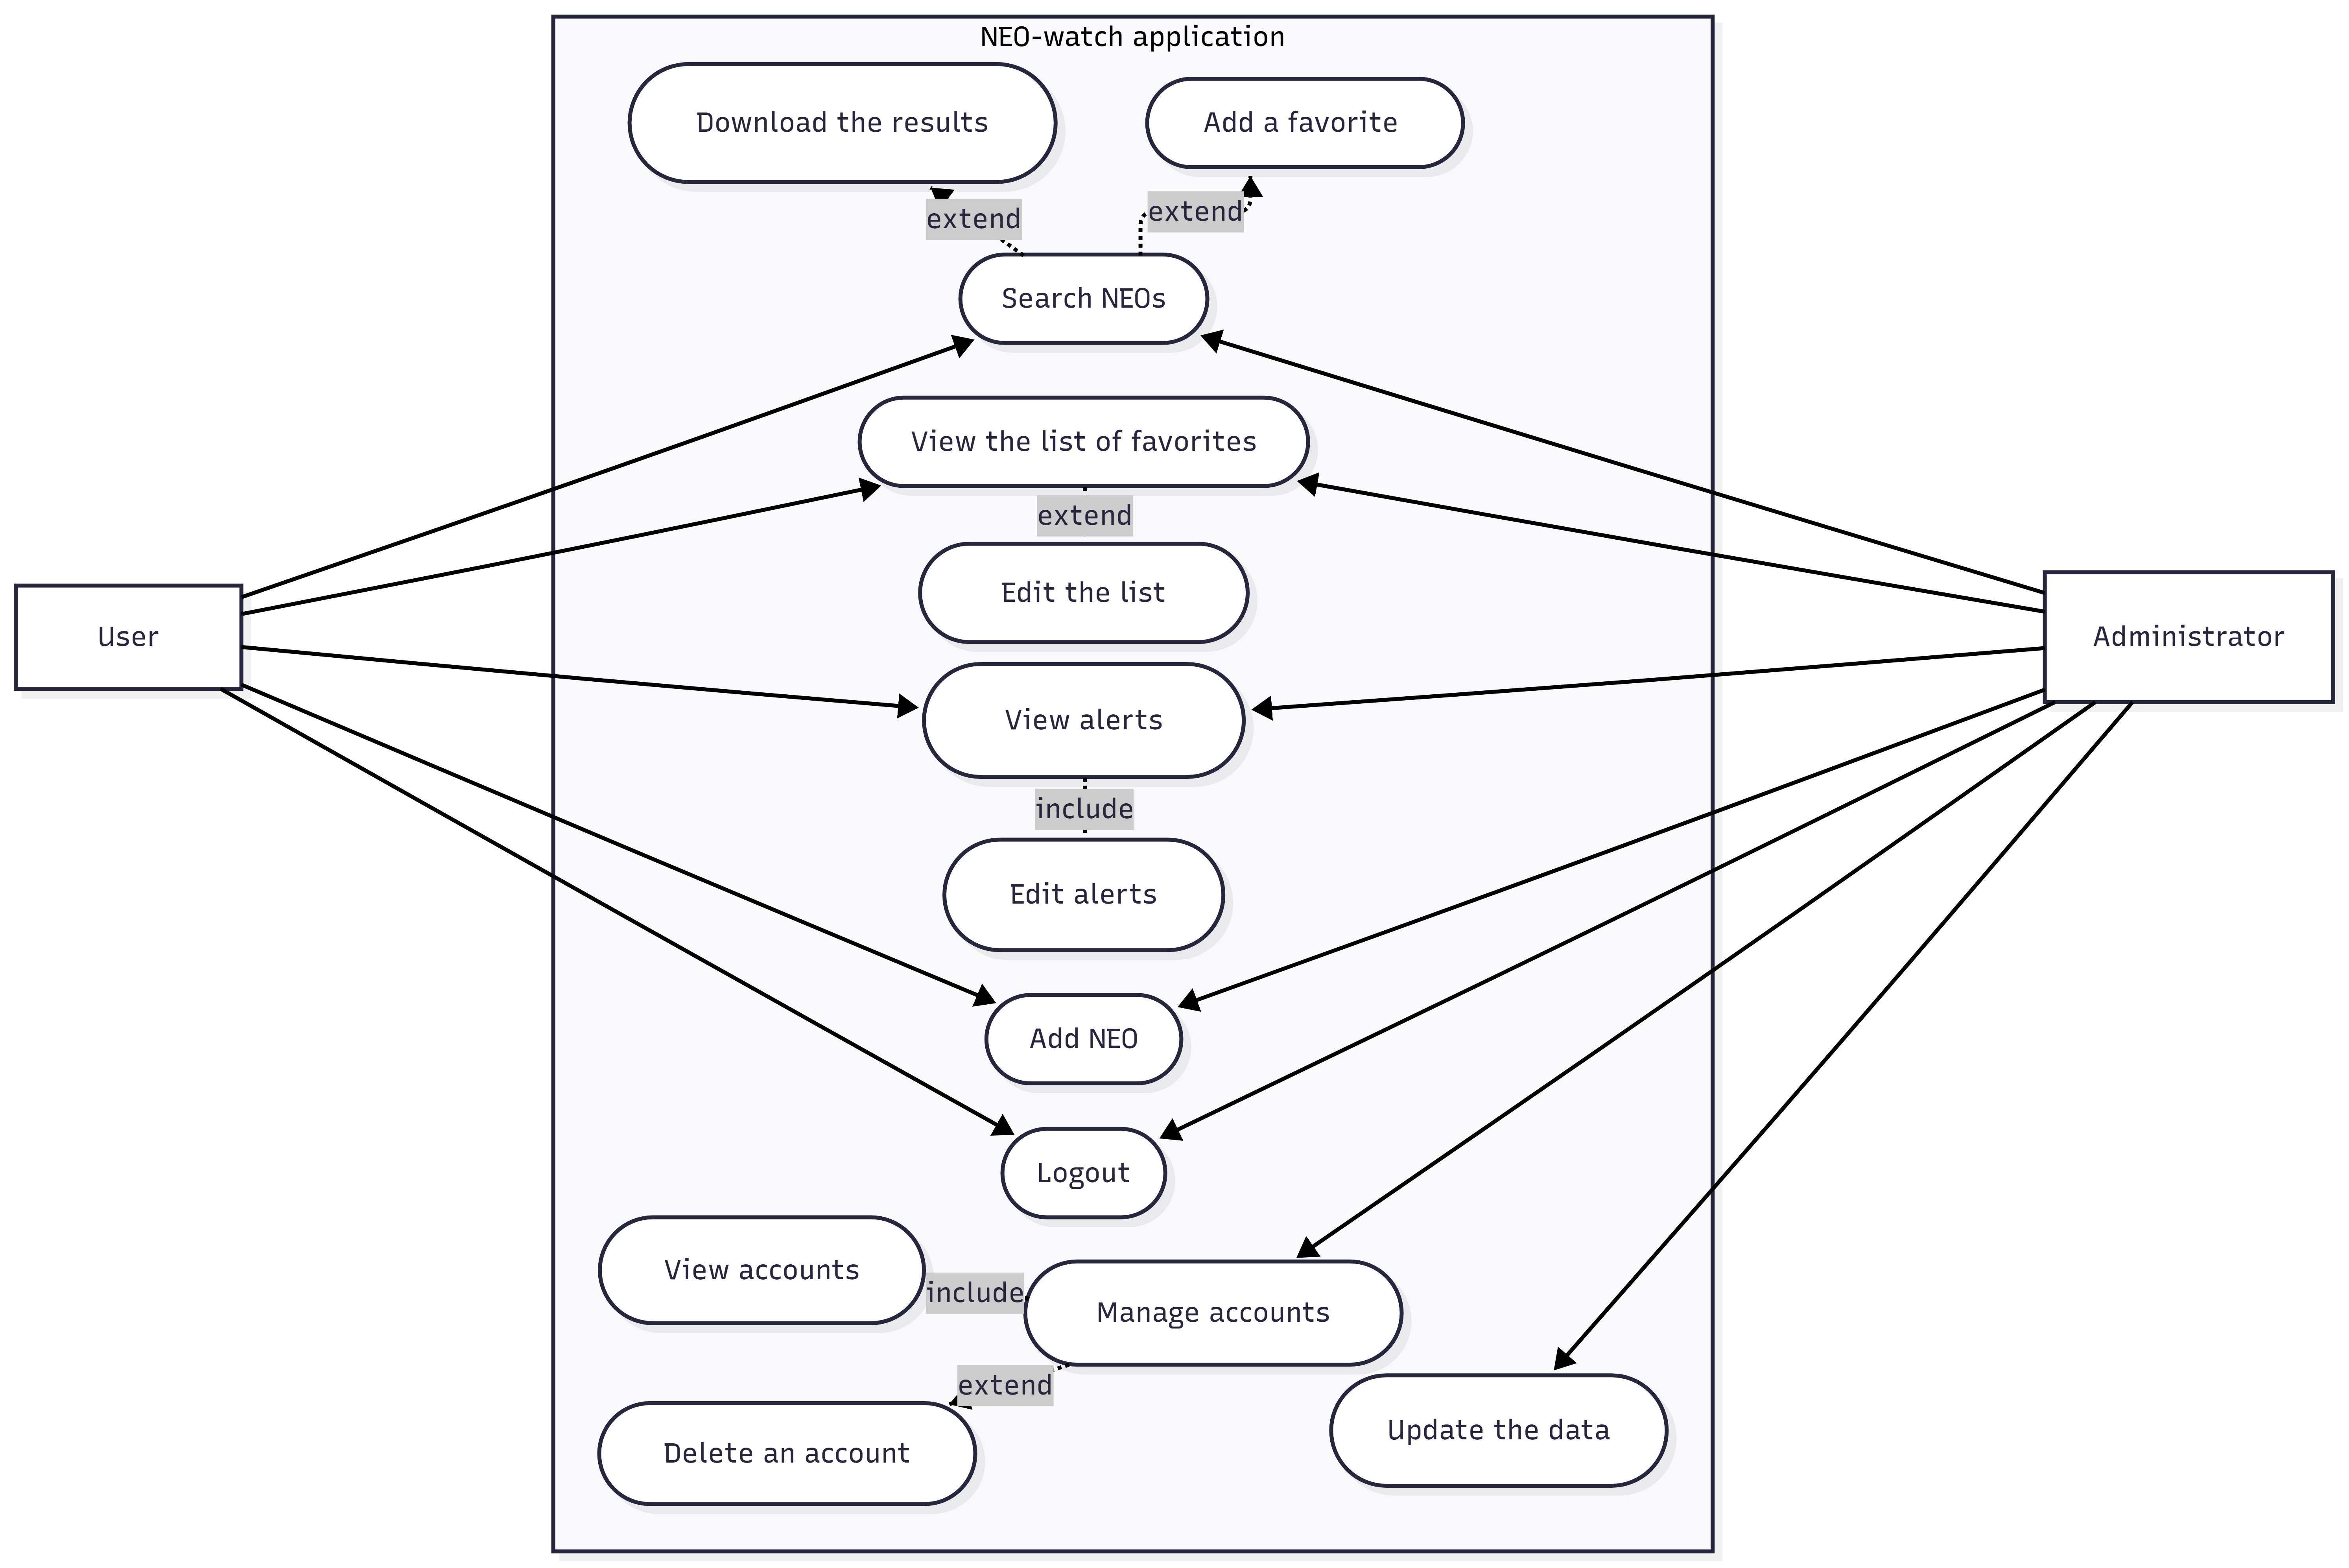
\includegraphics[keepaspectratio]{../doc/diagram/use_case_diagram.png}}

}

\caption{Use Case Diagram}

\end{figure}%

\chapter{II. Project organization and
planning}\label{ii.-project-organization-and-planning}

To ensure the successful completion of the implementation project, we
have decided to organise ourselves as follows.

We opted for a more flexible approach without assigning everyone a
specific role. This enabled us to understand every stage of the app's
development and to help one another. After agreeing on the app's overall
structure (analysis report), we divided up the various key features
amongst ourselves, from DAOs to controllers. As things progressed,
certain roles naturally fell into place. For example, Yann made sure
that the weekly tracking was updated regularly. This organisation ran
smoothly thanks to the small size of our team and good communication via
meetings and the WhatsApp group. At each meeting, we would list the
tasks we had completed and identify those that needed to be done before
the next deadline we had set ourselves, so that we could make steady
progress.

When it came to working as a team, GitHub proved to be a very useful
tool for keeping the project up to date and enabling us to work
simultaneously. By dividing the work into major features, we were able
to avoid file versioning conflicts.

\begin{figure}[H]

{\centering \pandocbounded{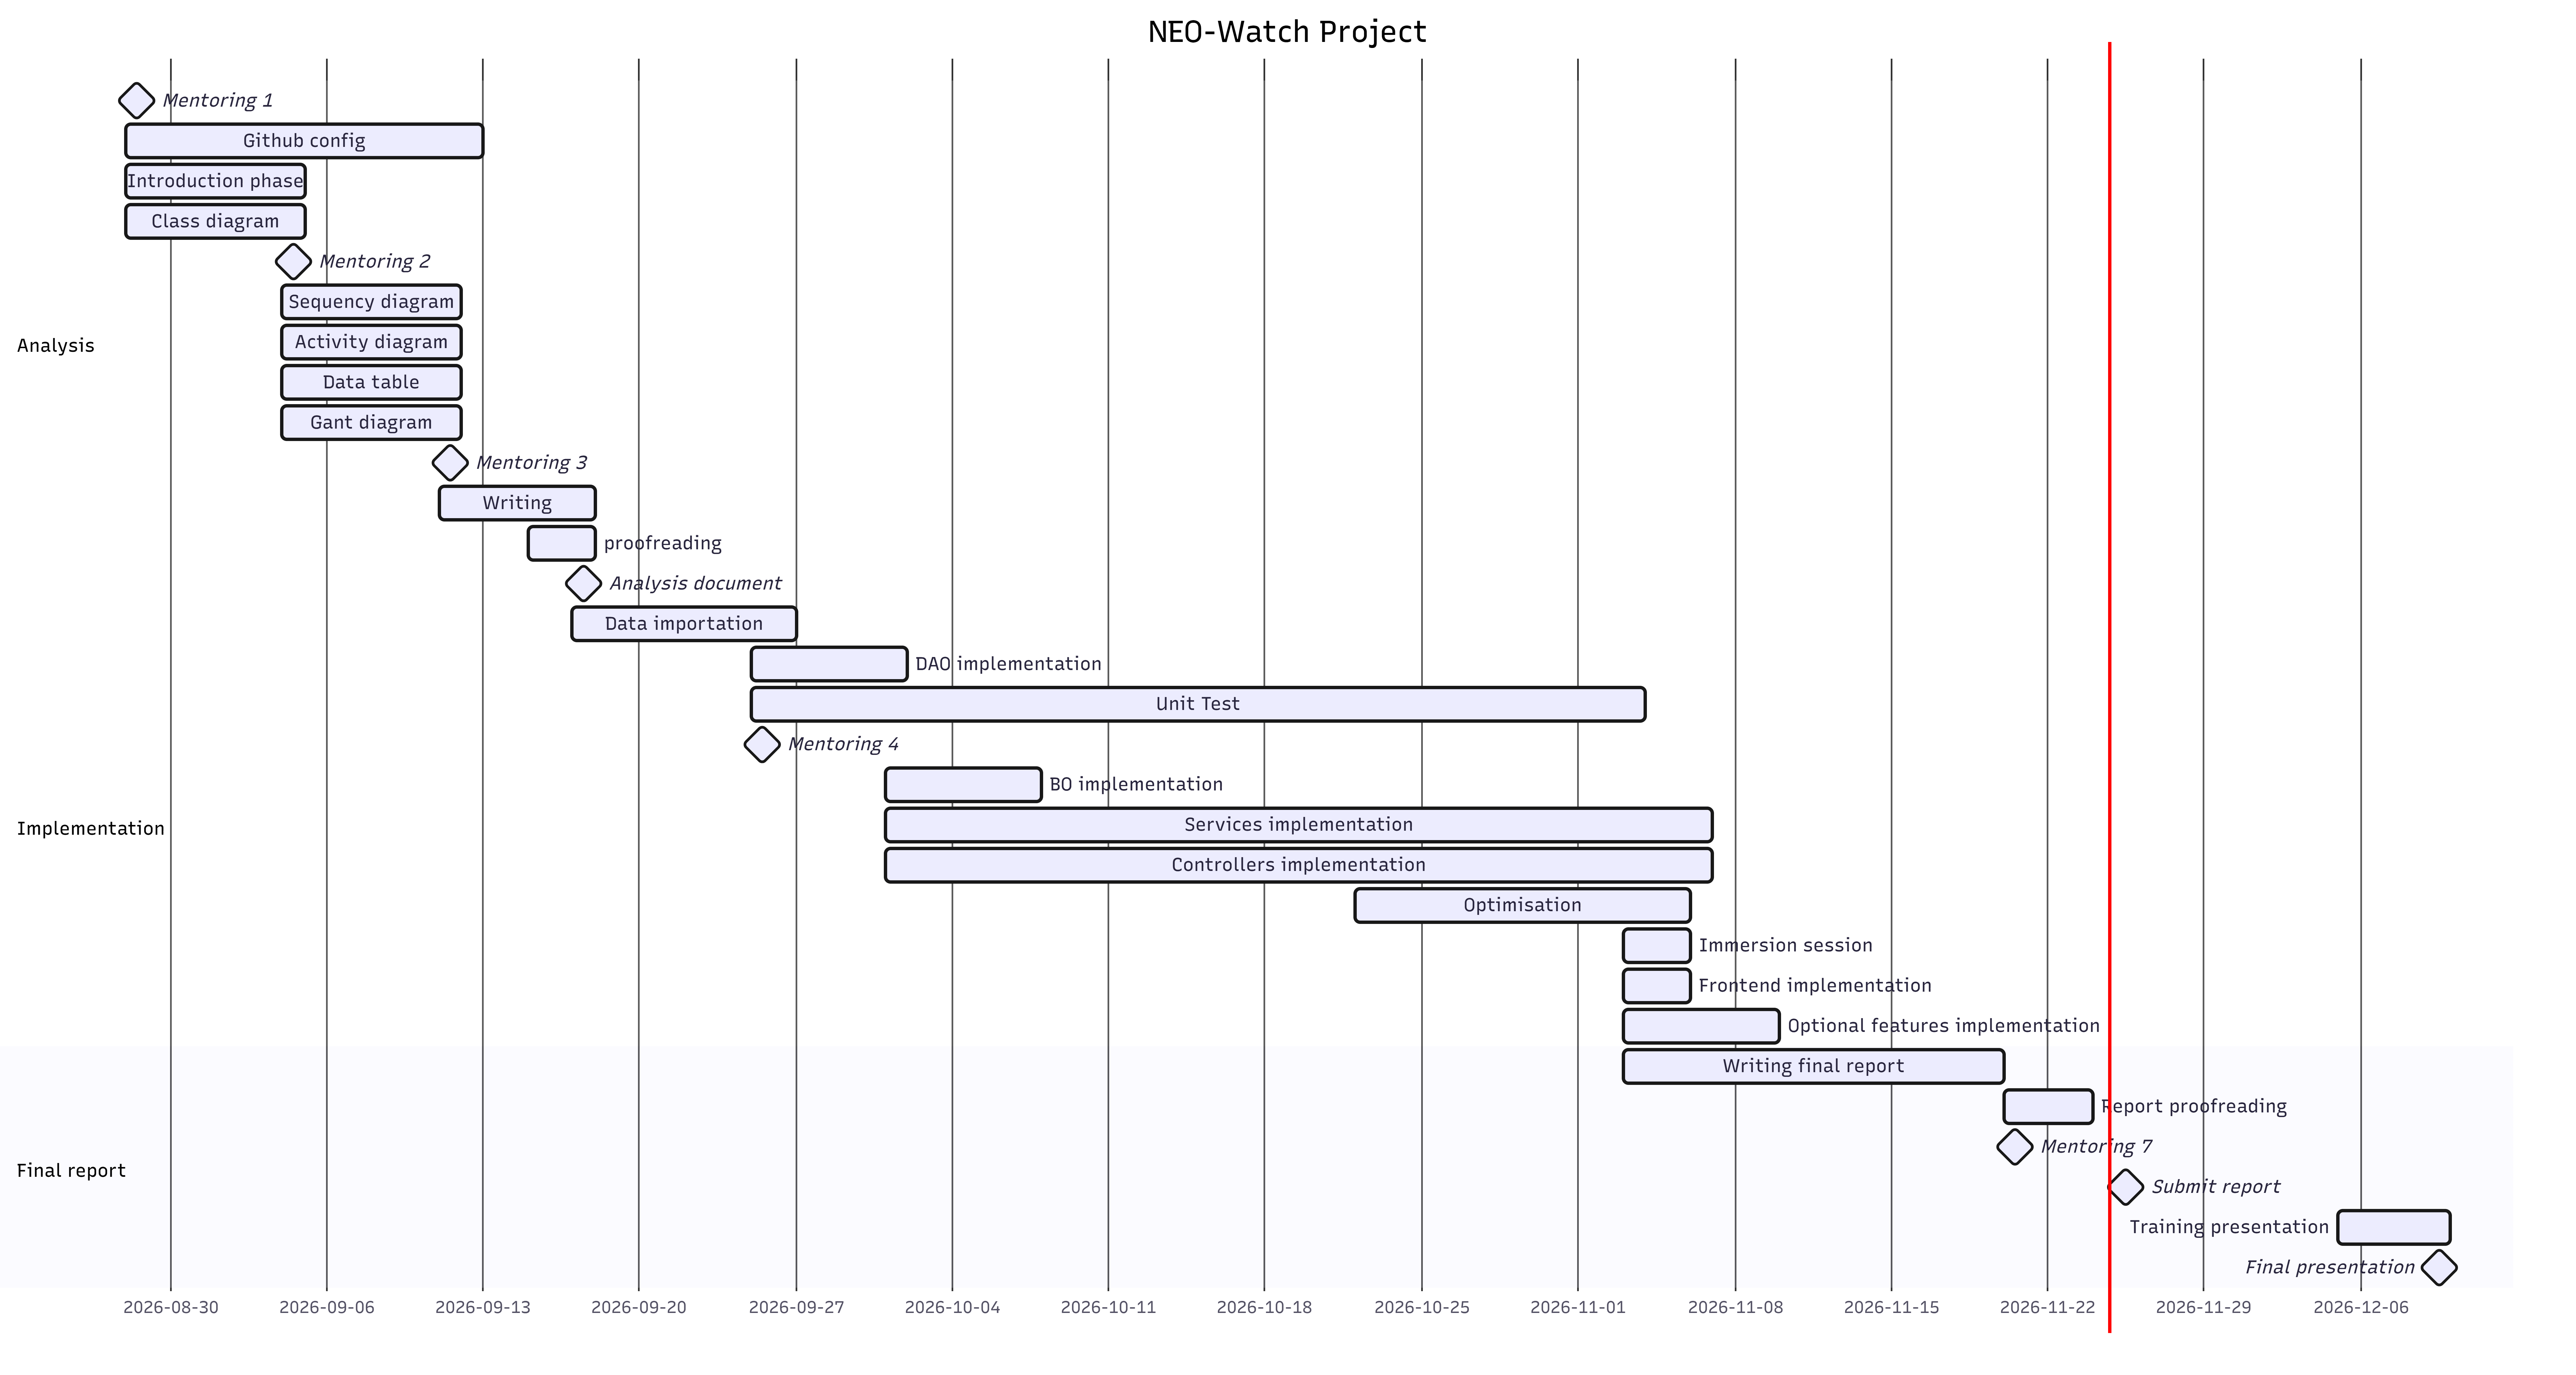
\includegraphics[keepaspectratio]{../doc/diagram/gantt_diagramal_vfinal.png}}

}

\caption{Gantt diagram}

\end{figure}%

\chapter{III. Application design}\label{iii.-application-design}

\section{A. Database}\label{a.-database}

The data about Near-Earth Objects (NEOs) is retrieved automatically
through the endpoints of NASA's NEO API. This API provides extensive
information about asteroids, including their orbital caractéristiques,
physical properties and close-approach predictions.

However, the API returns far more data than our application actually
needs. We therefore chose a selective approach: only information
considérés useful for the application is extracted and stored in the
database. This includes the NASA identifier, the object's name, its
estimated diameter range, its absolute magnitude and esther it is
classified as potentially hazardons, along with the details of its close
approaches to Earth (date, orbitant body, miss distance and relative
velocity). This deliberate filtering keeps the database lightweight,
simplifies queries and avoids storing redundant or unused fields.

\begin{figure}[H]

{\centering \pandocbounded{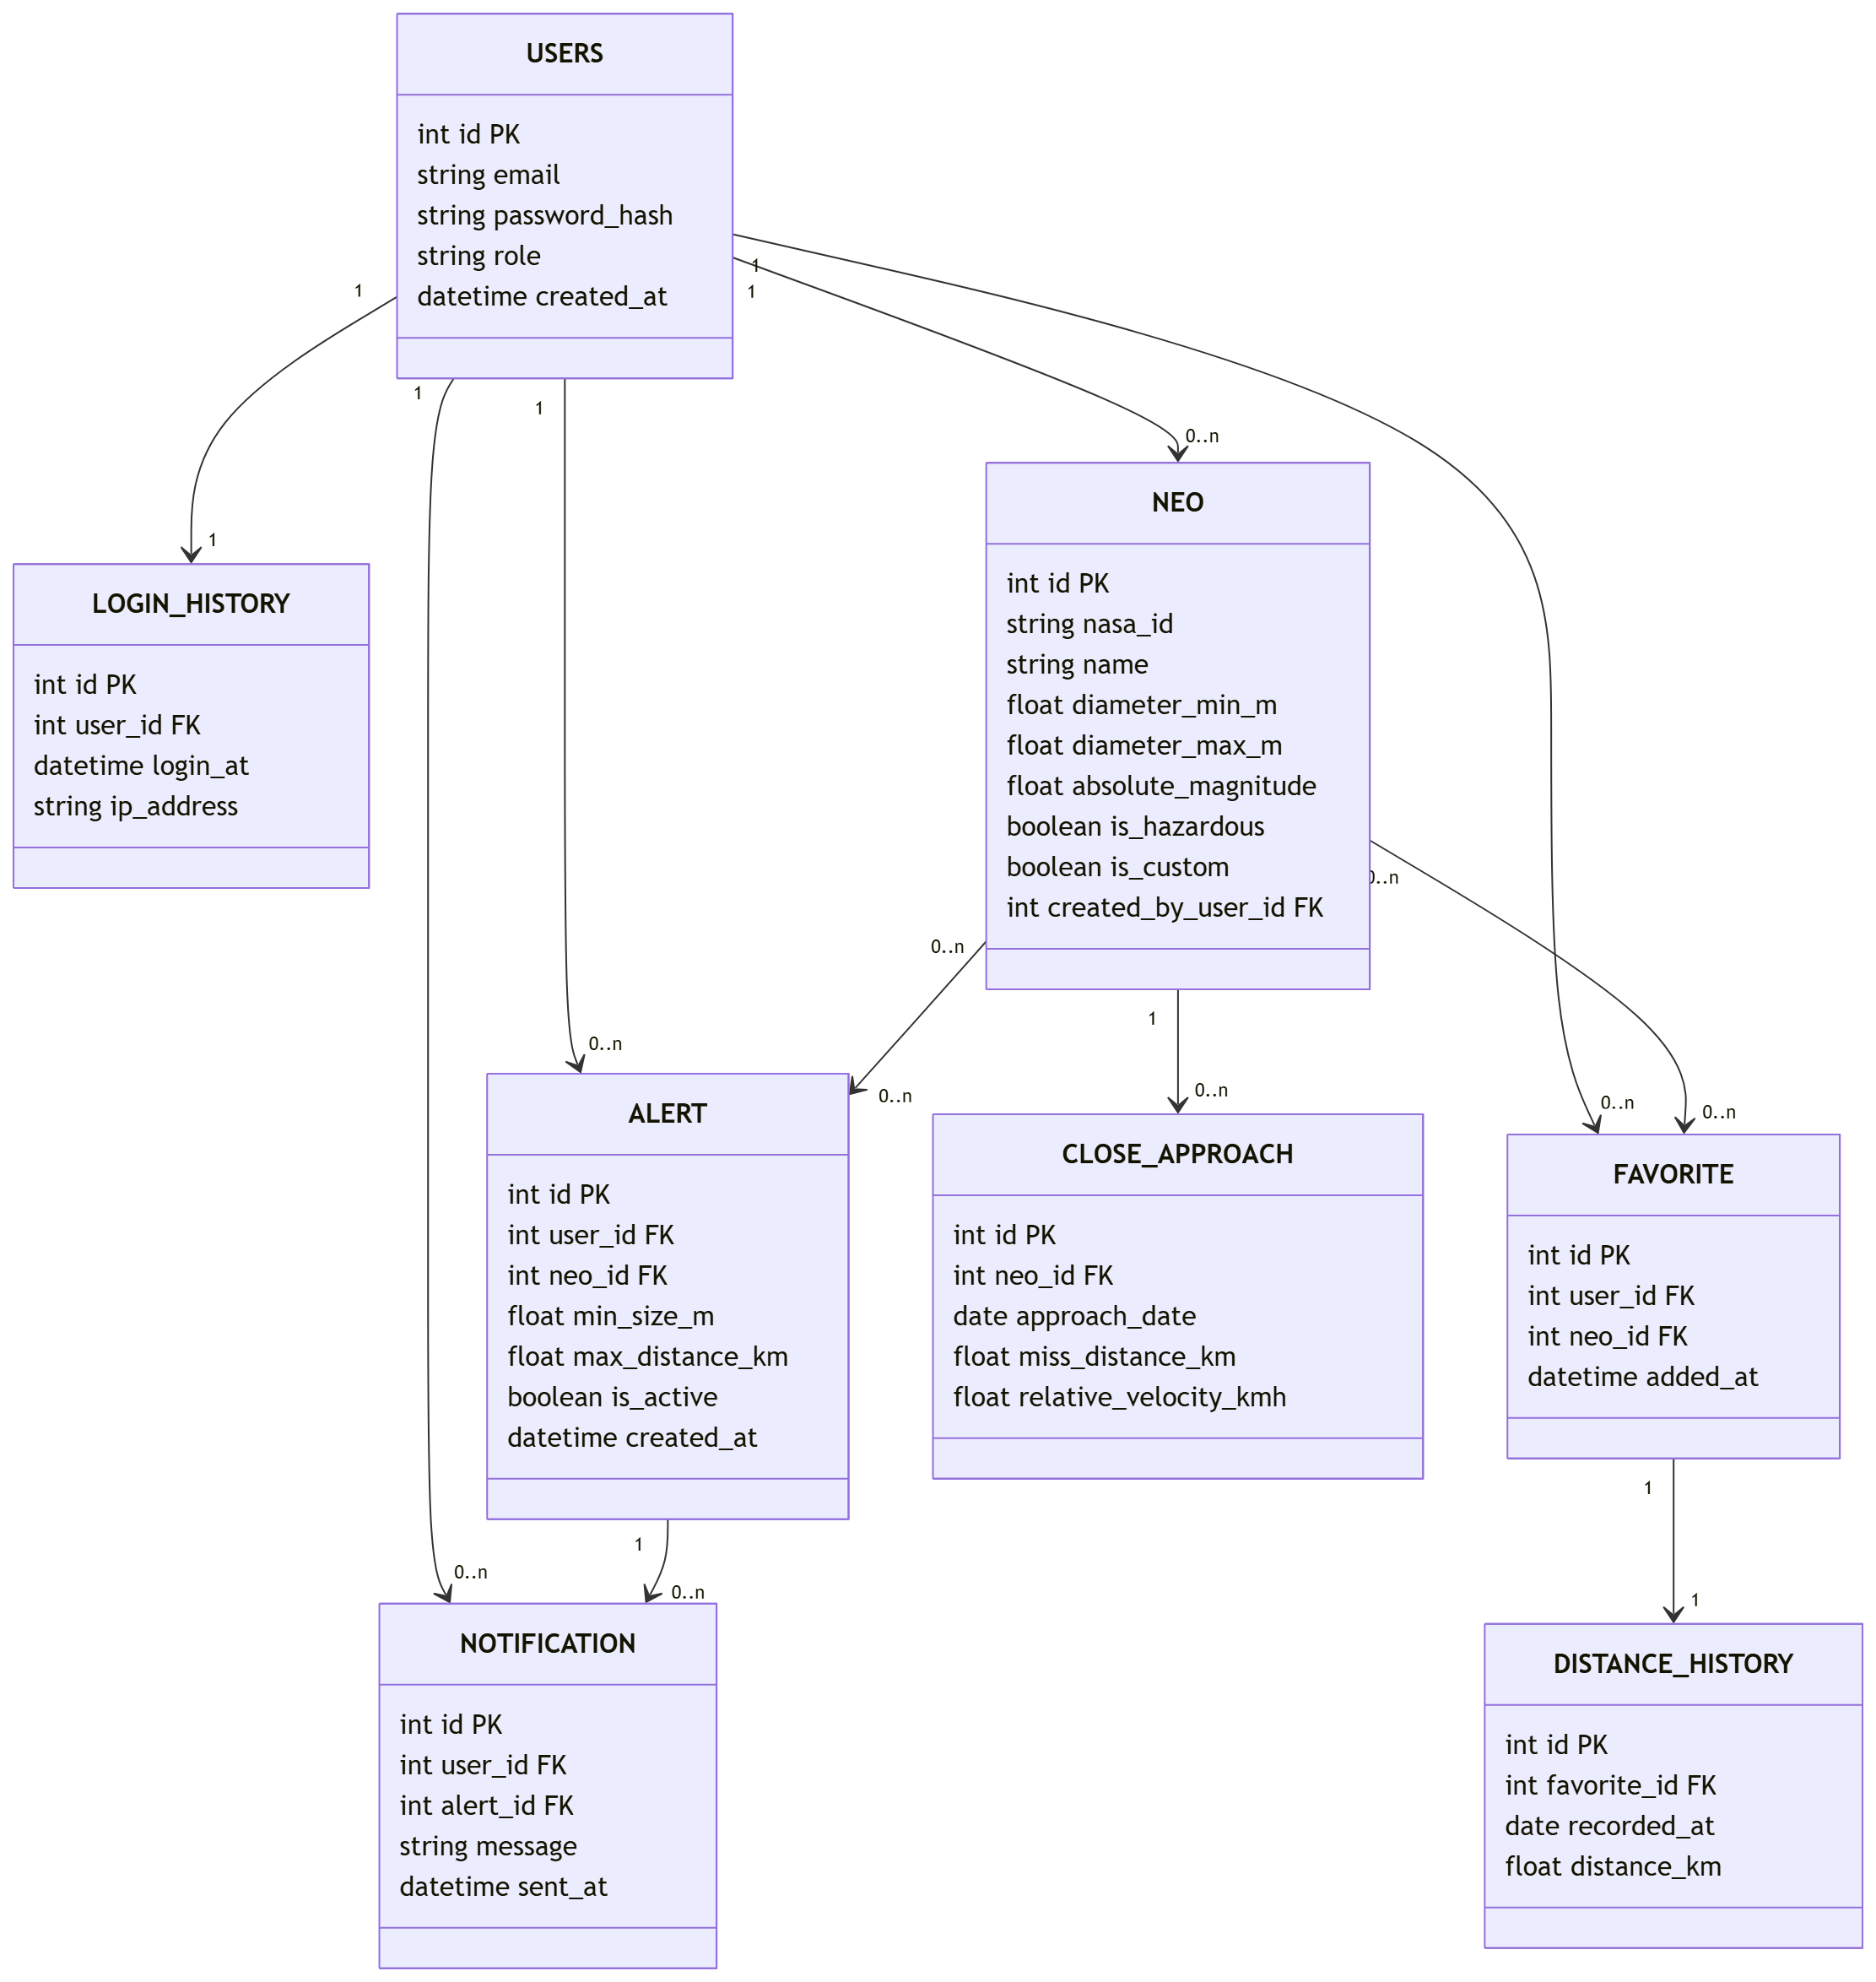
\includegraphics[keepaspectratio]{../doc/diagram/diagram_bdd.png}}

}

\caption{Table Diagram}

\end{figure}%

The database is organized around two central entities (\texttt{users}
and \texttt{neo}) with all other tables depending on them through
foreign keys. As shown in the table diagram (figure ?), every
relationship follows a one-to-many (1 : N) pattern, with a single
exception.

The \texttt{users} table anchors account management. It connects to
\texttt{login\_history} when the user log in, \texttt{alert} when they
are configured, \texttt{favorite} when the user adds a neo as a
favorite, and \texttt{neo} when he creates its own NEOs.

The \texttt{neo} table anchors the astronomical data. It connects to
\texttt{close\_approach} the close approach history of a NEO,
\texttt{favorite} where a NEO can be saved by a user and \texttt{alert}
to trigger them when they are configured by users.

The only deviation from the standard pattern is the \texttt{neo} and
\texttt{alert} link: since \texttt{alert.id\_neo} is nullable, an alert
can either target a specific NEO (0..1 : N) or be generic and triggered
by any object crossing the configured thresholds.

In short, the schema separates who uses the application (\texttt{users},
\texttt{login\_history}), what is observed (\texttt{neo},
\texttt{close\_approach}) and how users interact with data
(\texttt{alert}, \texttt{favorite}, \texttt{distance\_history}).

To store this database, we use PostgreSQL which we connect to via the
\texttt{.env} file. This system allows multiple users to view and edit
the database at the same time.

\textbf{Database updates.} Because NASA continuously refines orbital
parameters and publishes new close-approach predictions, the local
PostgreSQL database must be refreshed periodically without disrupting
active users or overwriting custom asteroids. Rather than querying
NASA's API on every user request, updates are triggered explicitly by an
administrator through the \texttt{POST\ /admin/import} endpoint.

The update workflow relies on a dedicated synchronization script
(\texttt{utils.weekly\_data}) executed in an isolated background
subprocess (\texttt{subprocess.run}) so that the API remains responsive
and immediately returns a \texttt{202\ Accepted} status. To prevent
concurrent writes or duplicate API bursts, a shared thread lock
(\texttt{threading.Lock}) ensures that only one synchronization runs at
a time, rejecting overlapping requests with a \texttt{409\ Conflict}
error.

Because NASA's \texttt{/feed} endpoint restricts queries to a seven-day
window, \texttt{sync\_weekly\_feed} computes a rolling seven-day
interval ending on the current date (\texttt{end\ -\ 6\ days} to
\texttt{end}) and delegates the ingestion to
\texttt{NeoService.sync\_nasa\_data}. For each retrieved object, the
service performs a non-destructive upsert:

\begin{itemize}
\tightlist
\item
  \textbf{Existing NASA NEOs} (matched by \texttt{nasa\_id}) have their
  physical and orbital attributes updated without altering their
  internal primary key (\texttt{id\_neo}), preserving existing user
  alerts and favorites.
\item
  \textbf{Close approaches} are deduplicated against existing
  \texttt{(id\_neo,\ orbiting\_body,\ approach\_date)} records so that
  repeated runs only insert newly detected flybys.
\item
  \textbf{User-created NEOs} (\texttt{is\_custom\ =\ True}) carry
  synthetic identifiers (\texttt{CUSTOM-...}) and are never touched by
  the synchronization process, guaranteeing full data integrity across
  updates.
\end{itemize}

\section{B. Architecture}\label{b.-architecture}

Our project is a client-server application. The client (frontend) and
the server (backend) communicate through HTTP requests and exchange data
in JSON format. The application is built around four major components.

\textbf{Backend}

Developed in Python, the backend centralizes the application logic. It
follows the classic layered model seen in class, in order to strictly
separate responsibilities:

\begin{itemize}
\tightlist
\item
  Controllers \& schemas: expose the API endpoints through routers and
  handle the HTTP requests coming from the client.
\item
  Services \& business objects: the core of the system. They contain all
  the business logic, such as alert processing, favorites management and
  the creation of objects.
\item
  DAO: the software layer dedicated to interactions with the PostgreSQL
  database. Client: the code that communicates with the NASA API.
\end{itemize}

\textbf{Frontend}

Developed in Python with the Streamlit library, which makes it possible
to generate interactive dashboards. It collects the user's actions and
displays the data.

\textbf{Internal database}

We use the PostgreSQL relational database management system, which
ensures the integrity of our data.

\textbf{External data source}

To feed the application, the backend retrieves data from the NASA NeoWs
API. The data is then filtered, transformed and inserted into our own
PostgreSQL database.

Architecture diagram

\begin{figure}[H]

{\centering \pandocbounded{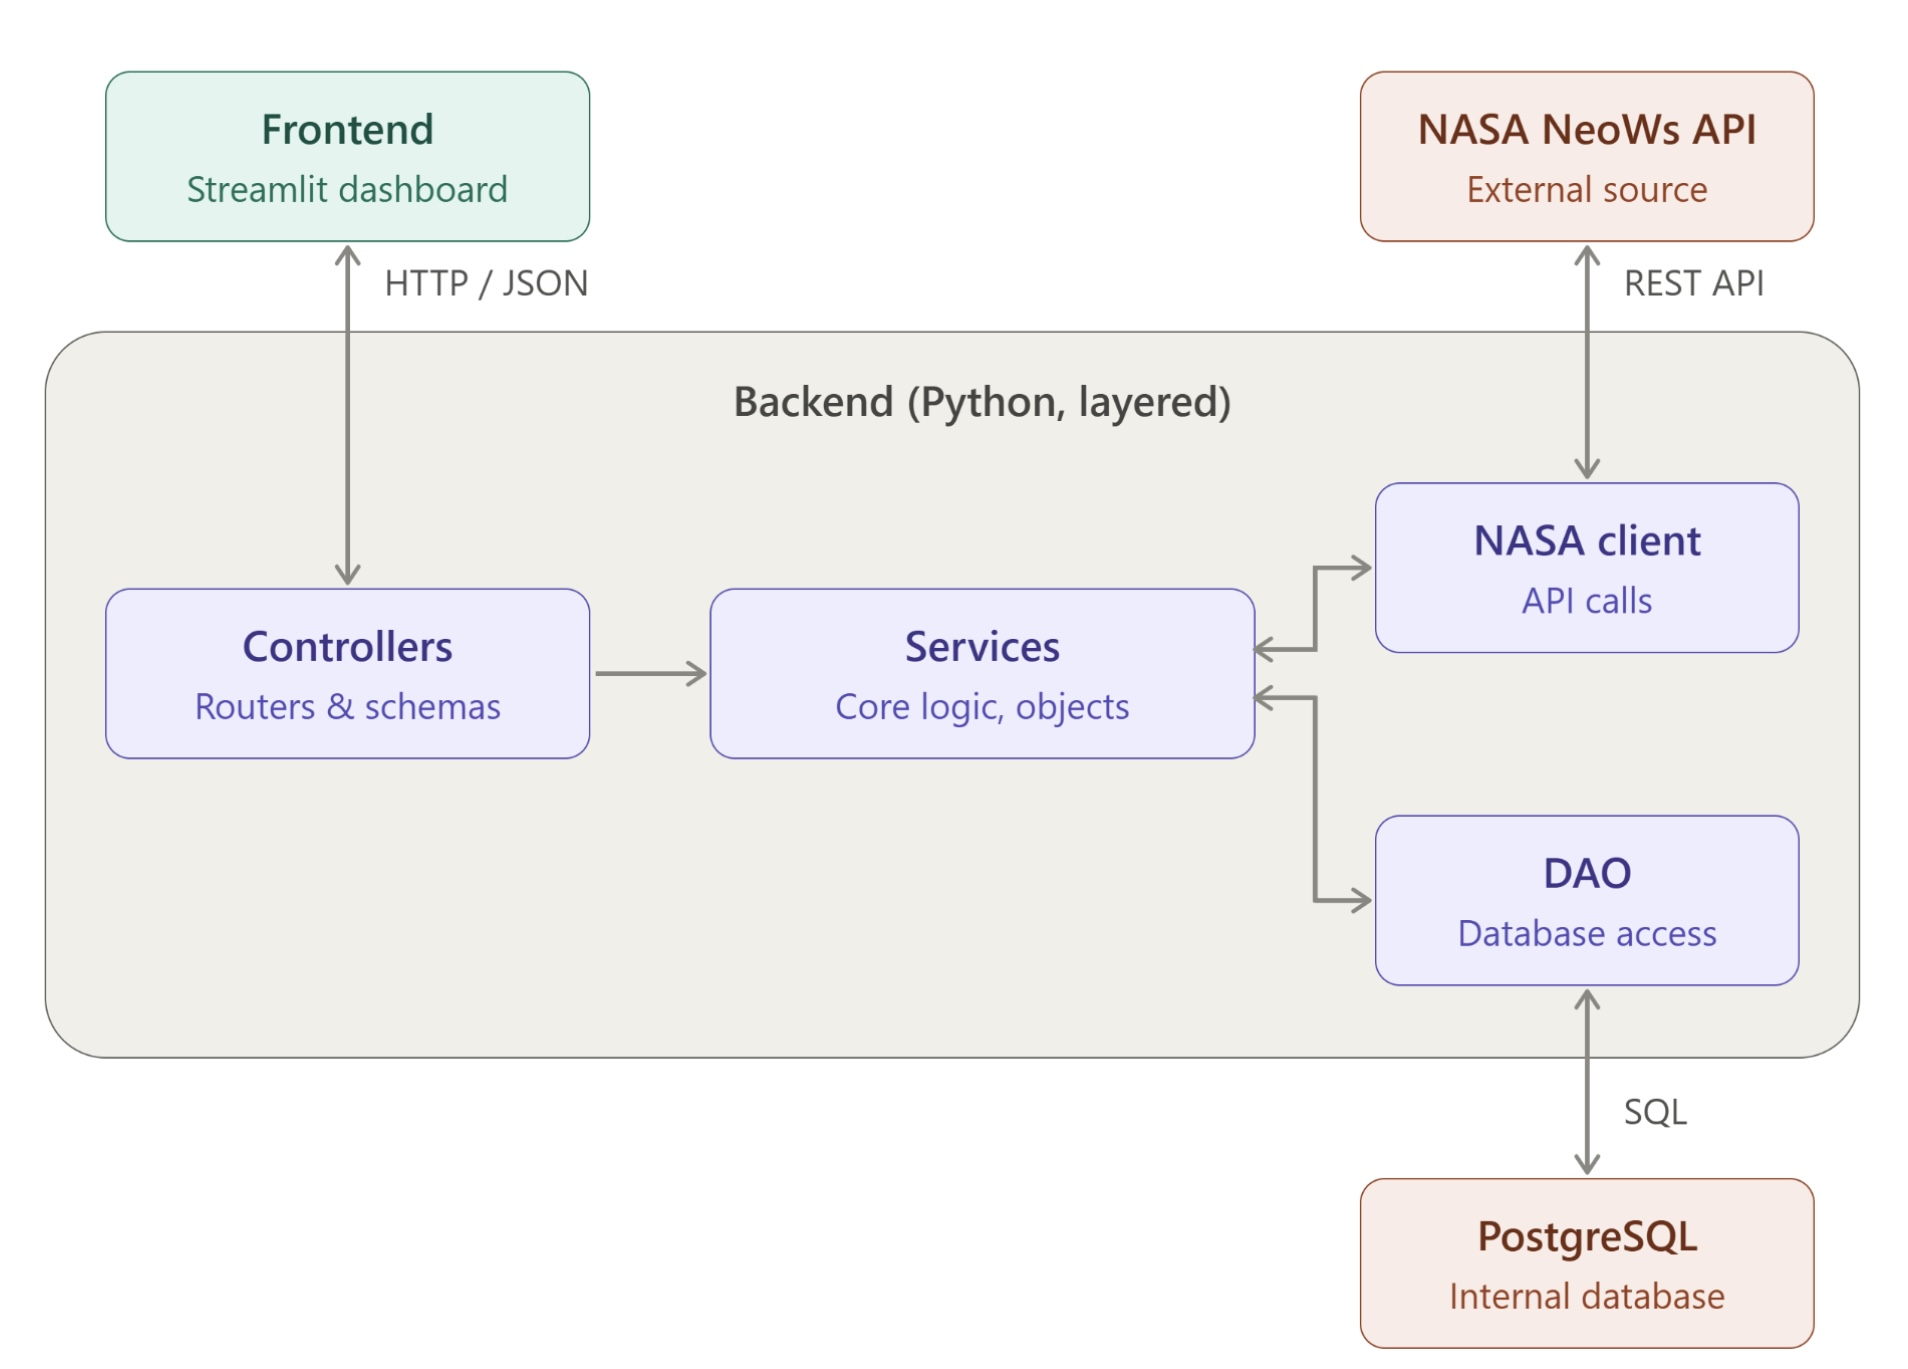
\includegraphics[keepaspectratio]{../doc/diagram/architecture_diagram.jpeg}}

}

\caption{Architecture Diagram}

\end{figure}%

\section{C. Features' implementation}\label{c.-features-implementation}

All features follow the same structure: the layered architecture. The
Pydantic models (\texttt{schema/}) are separate from the business
objects: for example, \texttt{UserResponseModel} never contains
\texttt{password\_hash} or \texttt{token}, so sensitive data cannot leak
through API responses. Each section below presents the endpoints (with
the required access level) followed by the design choices of the
feature.

\subsection{1. User (/users)}\label{user-users}

{\def\LTcaptype{none} % do not increment counter
\begin{longtable}[]{@{}
  >{\raggedright\arraybackslash}p{(\linewidth - 8\tabcolsep) * \real{0.2000}}
  >{\raggedright\arraybackslash}p{(\linewidth - 8\tabcolsep) * \real{0.2000}}
  >{\raggedright\arraybackslash}p{(\linewidth - 8\tabcolsep) * \real{0.2000}}
  >{\raggedright\arraybackslash}p{(\linewidth - 8\tabcolsep) * \real{0.2000}}
  >{\raggedright\arraybackslash}p{(\linewidth - 8\tabcolsep) * \real{0.2000}}@{}}
\toprule\noalign{}
\begin{minipage}[b]{\linewidth}\raggedright
Endpoint
\end{minipage} & \begin{minipage}[b]{\linewidth}\raggedright
Purpose
\end{minipage} & \begin{minipage}[b]{\linewidth}\raggedright
Access
\end{minipage} & \begin{minipage}[b]{\linewidth}\raggedright
Success
\end{minipage} & \begin{minipage}[b]{\linewidth}\raggedright
Errors
\end{minipage} \\
\midrule\noalign{}
\endhead
\bottomrule\noalign{}
\endlastfoot
POST /users/ & Account creation & Public & 201 + user & 422 (invalid
data), 500 (insertion failed) \\
POST /users/logout & Close the session & Token required & 204 & 401
(unknown or already closed token) \\
GET /users/me & Profile of the logged-in user & Token required & 200 +
user & 401 (via the dependency) \\
\end{longtable}
}

\textbf{Registration.} The service normalizes the email (lower case,
surrounding spaces removed), checks its format, the password length (8
characters minimum) and the uniqueness of the email. The password is
never stored in clear text. It is hashed with a random salt unique to
each user. The salt and the iteration count are stored inside the hash
string, so these parameters can evolve without breaking existing
accounts.

\textbf{Logout and authentication.} A session is a random token
(\texttt{secrets.token\_urlsafe}) stored in the \texttt{users} table.
Logging out sets this token back to \texttt{None}. On every protected
request, \texttt{authenticate} finds the user by token and refuses
access if the user is banned, so a ban takes effect immediately without
waiting for a session to expire.

\begin{figure}[H]

{\centering \pandocbounded{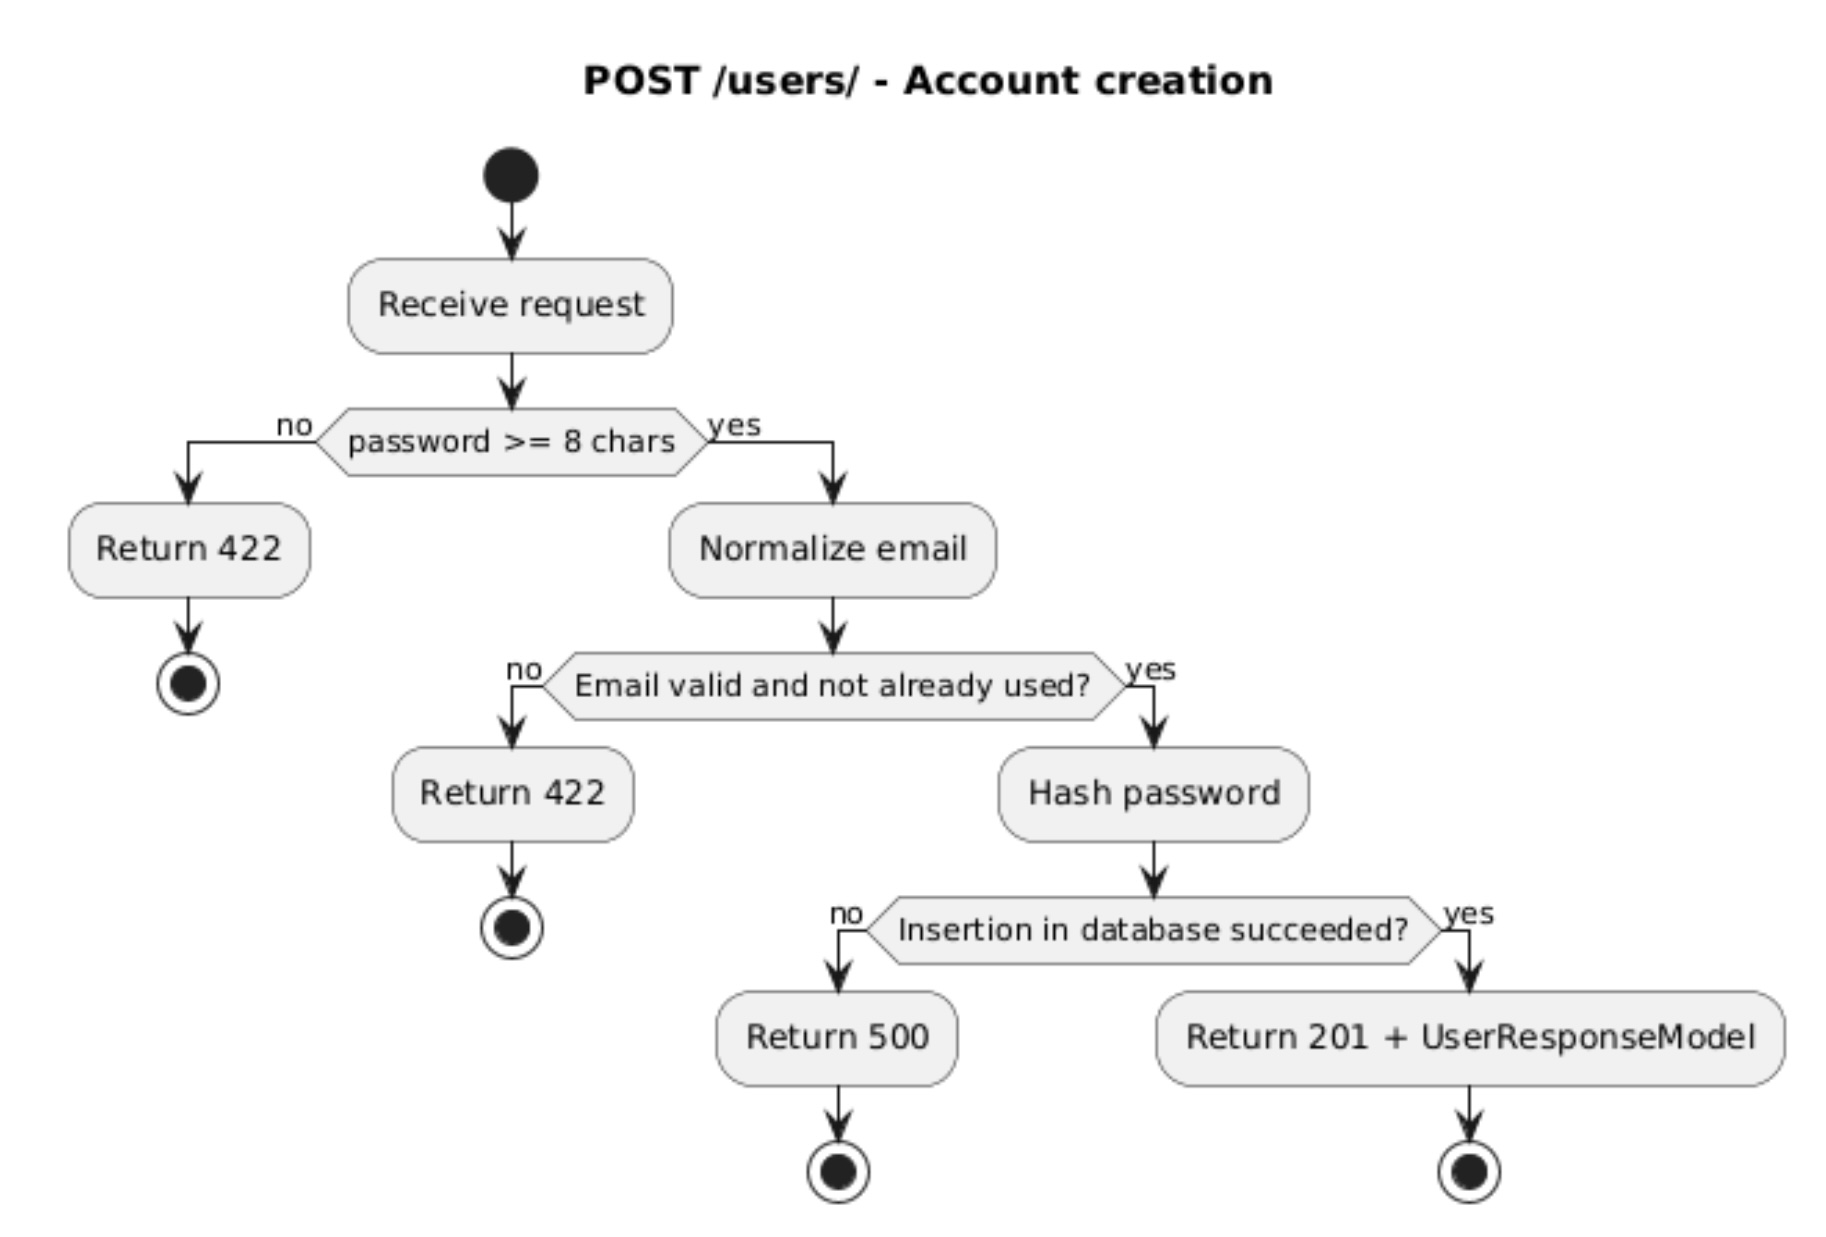
\includegraphics[keepaspectratio]{../doc/diagram/endpoint_post_users_diagram.jpeg}}

}

\caption{Activity diagram for POST/users/ endpoint}

\end{figure}%

\subsection{2. Admin (/admin)}\label{admin-admin}

{\def\LTcaptype{none} % do not increment counter
\begin{longtable}[]{@{}
  >{\raggedright\arraybackslash}p{(\linewidth - 8\tabcolsep) * \real{0.2667}}
  >{\raggedright\arraybackslash}p{(\linewidth - 8\tabcolsep) * \real{0.2000}}
  >{\raggedright\arraybackslash}p{(\linewidth - 8\tabcolsep) * \real{0.1333}}
  >{\raggedright\arraybackslash}p{(\linewidth - 8\tabcolsep) * \real{0.2000}}
  >{\raggedright\arraybackslash}p{(\linewidth - 8\tabcolsep) * \real{0.2000}}@{}}
\toprule\noalign{}
\begin{minipage}[b]{\linewidth}\raggedright
Endpoint
\end{minipage} & \begin{minipage}[b]{\linewidth}\raggedright
Purpose
\end{minipage} & \begin{minipage}[b]{\linewidth}\raggedright
Access
\end{minipage} & \begin{minipage}[b]{\linewidth}\raggedright
Success
\end{minipage} & \begin{minipage}[b]{\linewidth}\raggedright
Errors
\end{minipage} \\
\midrule\noalign{}
\endhead
\bottomrule\noalign{}
\endlastfoot
POST /admin/users/\{id\_user\}/ban & Ban a user & Admin & 204 & 400
(unknown user, admin, or self), 500 \\
POST /admin/import & Start the NASA data import & Admin & 202 & 409
(import already running) \\
GET /admin/connections & Connection history (filterable by id\_user) &
Admin & 200 + list & 404 (unknown user) \\
\end{longtable}
}

\textbf{Access control.} Rights are checked at two levels: the
\texttt{require\_admin} dependency in the controller, and
\texttt{\_require\_admin} in the service. The service therefore stays
protected even if it is called from an entry point other than the API.

\textbf{Ban.} The service refuses self-bans and bans of other admins. It
sets \texttt{is\_banned} to \texttt{True} and removes the token, which
closes the current session. The user cannot log in again, since login
refuses banned accounts.

\textbf{Data import.} This is the most interesting feature technically,
because the import to update the data is long (timeout set to 1 hour).
Three design choices:

\begin{itemize}
\tightlist
\item
  the import runs in a subprocess (\texttt{subprocess.run}), isolated
  from the API, with a timeout;
\item
  the endpoint immediately returns \texttt{202\ Accepted} and delegates
  the work to a FastAPI \texttt{BackgroundTask}, whose outcome only
  appears in the logs;
\item
  a lock (\texttt{threading.Lock}, shared between instances) ensures
  that only one import runs at a time. The controller checks
  \texttt{is\_import\_running()} to return 409, and the service also
  performs a non-blocking acquire. This second protection covers the
  case where two requests arrive simultaneously.
\end{itemize}

\textbf{Connection history.} The endpoint delegates to the history
service (all users, or a single user after checking that they exist).
This history feeds the connections section.

\subsection{3. Login and connections (/login,
/connections)}\label{login-and-connections-login-connections}

Login checks who the user is and opens a session; connection history
keeps a trace of every successful login, which the administrator can
consult.

{\def\LTcaptype{none} % do not increment counter
\begin{longtable}[]{@{}
  >{\raggedright\arraybackslash}p{(\linewidth - 8\tabcolsep) * \real{0.2000}}
  >{\raggedright\arraybackslash}p{(\linewidth - 8\tabcolsep) * \real{0.2000}}
  >{\raggedright\arraybackslash}p{(\linewidth - 8\tabcolsep) * \real{0.2000}}
  >{\raggedright\arraybackslash}p{(\linewidth - 8\tabcolsep) * \real{0.2000}}
  >{\raggedright\arraybackslash}p{(\linewidth - 8\tabcolsep) * \real{0.2000}}@{}}
\toprule\noalign{}
\begin{minipage}[b]{\linewidth}\raggedright
Endpoint
\end{minipage} & \begin{minipage}[b]{\linewidth}\raggedright
Purpose
\end{minipage} & \begin{minipage}[b]{\linewidth}\raggedright
Access
\end{minipage} & \begin{minipage}[b]{\linewidth}\raggedright
Success
\end{minipage} & \begin{minipage}[b]{\linewidth}\raggedright
Errors
\end{minipage} \\
\midrule\noalign{}
\endhead
\bottomrule\noalign{}
\endlastfoot
POST /login/ & Check the credentials, open a session and record the
connection & Public & 200, with \texttt{id\_user} and
\texttt{access\_token} & 401 (wrong email or password, or banned
user) \\
GET /connections/ & List the connections: all of them for an
administrator, only his own for a regular user & Token required & 200,
list of connections & 401 (missing or invalid token), 404 (no
connection) \\
GET /connections/users/\{id\_user\} & List the connections of one user &
Token required & 200, list of connections & 404 (no connection for this
user) \\
\end{longtable}
}

A connection is returned as \texttt{id\_login}, \texttt{id\_user} and
\texttt{login\_at} (the date and time of the login), described by the
\texttt{ConnectionReadModel} schema. Like the \texttt{UserResponseModel}
of the user feature, this schema is separate from the business object,
so only the intended fields leave the API.

\textbf{How a login works.} The client sends the email and the password.
The controller gives them to \texttt{UserService.login}, which does all
the checking. Only if the login succeeds does the controller call
\texttt{ConnectionHistoryService.create} to record the connection, and
then it returns the token. Several choices here are worth explaining:

\begin{itemize}
\tightlist
\item
  \textbf{Same answer for every refusal.} An unknown email, a wrong
  password and a banned account all give the same
  \texttt{401\ Invalid\ credentials}. An attacker cannot use the
  application to find out which emails have an account, or which
  accounts are banned. The ban is checked after the password for the
  same reason.
\item
  \textbf{A salted hash, compared in constant time.} The stored password
  is a PBKDF2-SHA256 hash with a random salt. The comparison uses
  \texttt{hmac.compare\_digest}, whose duration does not depend on how
  many characters match.
\item
  \textbf{The history never blocks the login.} Recording the connection
  is secondary information. If it fails (for example if the database
  refuses the insertion), the error is written in the logs and the user
  is still logged in.
\item
  \textbf{A new token at each login.} The token is generated with
  \texttt{secrets.token\_urlsafe}, the standard module for secrets, and
  replaces the previous one.
\end{itemize}

\textbf{How a protected request is checked.} After the login, the client
sends the token in the header
\texttt{Authorization:\ Bearer\ \textless{}token\textgreater{}}. Three
small functions of \texttt{dependencies.py} are chained by FastAPI
before the endpoint code runs:

\begin{itemize}
\tightlist
\item
  \texttt{get\_token} reads the header and answers
  \texttt{401\ Not\ authenticated} if it is missing.
\item
  \texttt{get\_current\_user} asks \texttt{UserService.authenticate} for
  the owner of the token. A token that does not exist, or whose user is
  banned, gives \texttt{401\ Invalid\ or\ expired\ token}.
\item
  \texttt{require\_admin} additionally answers
  \texttt{403\ Admin\ rights\ required} if the user is not an
  administrator.
\end{itemize}

The endpoint itself only receives the authenticated user and does not
repeat these checks. In \texttt{GET\ /connections/}, the same endpoint
serves both roles: the administrator receives every connection and the
regular user receives only his own, after filtering in the controller. A
regular user can therefore never read the history of someone else
through this endpoint. The token has no expiration date: a session ends
when the user logs out or when an administrator bans him, both of which
remove the token from the database.

\begin{figure}[H]

{\centering \pandocbounded{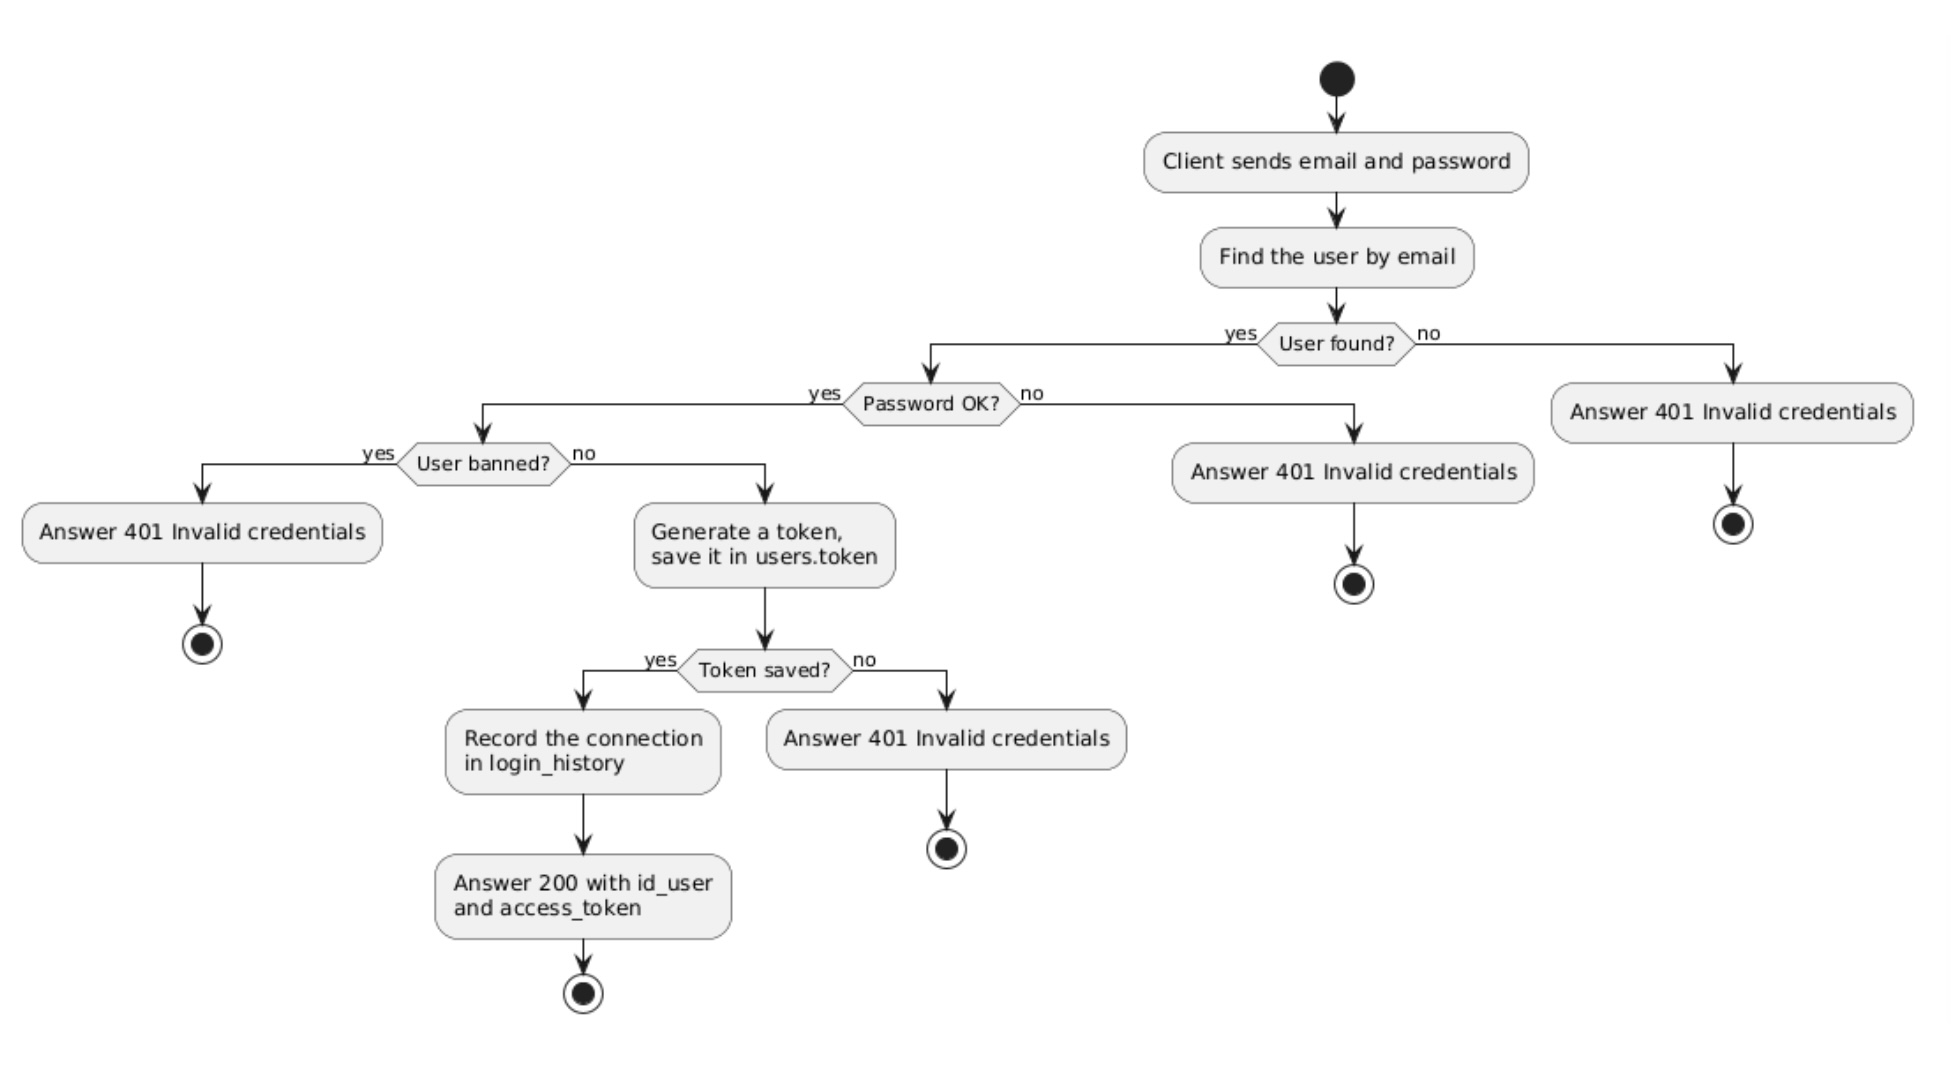
\includegraphics[keepaspectratio]{../doc/diagram/endpoint_post_login_diagram.jpeg}}

}

\caption{Activity diagram for POST/login/ endpoint}

\end{figure}%

\subsection{4. NEOs (/neo)}\label{neos-neo}

{\def\LTcaptype{none} % do not increment counter
\begin{longtable}[]{@{}
  >{\raggedright\arraybackslash}p{(\linewidth - 8\tabcolsep) * \real{0.2000}}
  >{\raggedright\arraybackslash}p{(\linewidth - 8\tabcolsep) * \real{0.2000}}
  >{\raggedright\arraybackslash}p{(\linewidth - 8\tabcolsep) * \real{0.2000}}
  >{\raggedright\arraybackslash}p{(\linewidth - 8\tabcolsep) * \real{0.2000}}
  >{\raggedright\arraybackslash}p{(\linewidth - 8\tabcolsep) * \real{0.2000}}@{}}
\toprule\noalign{}
\begin{minipage}[b]{\linewidth}\raggedright
Endpoint
\end{minipage} & \begin{minipage}[b]{\linewidth}\raggedright
Purpose
\end{minipage} & \begin{minipage}[b]{\linewidth}\raggedright
Access
\end{minipage} & \begin{minipage}[b]{\linewidth}\raggedright
Success
\end{minipage} & \begin{minipage}[b]{\linewidth}\raggedright
Errors
\end{minipage} \\
\midrule\noalign{}
\endhead
\bottomrule\noalign{}
\endlastfoot
GET /neo & Search NEOs (filters + optional sort) & Token required & 200
+ list & 400 (unknown sort key) \\
GET /neo/export & Export filtered NEOs as a CSV or JSON file & Token
required & 200 + file & 400 (unsupported format) \\
GET /neo/compare & Compare several NEOs and their closest Earth approach
& Token required & 200 + list & 404 (unknown NEO), 422 (fewer than 2
IDs) \\
GET /neo/nasa/\{nasa\_id\} & Get a NEO by its NASA identifier & Token
required & 200 & 404 (unknown \texttt{nasa\_id}) \\
GET /neo/\{id\_neo\} & Get a NEO by its id & Token required & 200 & 404
(unknown NEO) \\
GET /neo/\{id\_neo\}/close-approaches & List the close approaches of a
NEO & Token required & 200 + list & 404 (unknown NEO) \\
POST /neo & Create a custom NEO & Token required & 201 & 400 (missing
name) \\
DELETE /neo/\{id\_neo\} & Delete a NEO & Token required & 204 & 404
(unknown NEO) \\
POST /neo/sync/feed & Synchronize the NEOs of a date window (7 days max)
& Admin & 200 + summary & - \\
POST /neo/sync/page & Synchronize one page of the full NASA catalog &
Admin & 200 + summary & - \\
\end{longtable}
}

\textbf{Search.} Filtering happens in two stages inside
\texttt{search\_neos}: a filter runs in SQL with criterion as
\texttt{nasa\_id}, \texttt{user\_id}, or \texttt{is\_hazardous}, then
refined filtering runs in Python to combine all remaining criteria:
case-insensitive name substring, mean-diameter range, magnitude bound,
and close approaches via \texttt{CloseApproachDao}
(\texttt{orbiting\_body}, \texttt{approach\_date}). Sorting
(\texttt{sorting\_neo\_by}) is also done in Python, driven by the
\texttt{SORT\_KEYS} dictionary; NEOs with a missing value always come
last, and an unknown sort key returns 400.

\textbf{Export.} The service writes the \texttt{EXPORT\_FIELDS} fields
to a temporary file (CSV or JSON). The controller streams that file
through a \texttt{FileResponse} with a \texttt{BackgroundTask} that
deletes the temporary file once the response has been sent, so nothing
accumulates on disk.

\textbf{Comparison.} The controller exposes \texttt{GET\ /neo/compare},
relying on FastAPI's \texttt{Query(...,\ min\_length=2)} to enforce at
least two \texttt{ids} query parameters (automatically returning
\texttt{422} otherwise) and preserving the requested order. In
\texttt{NeoService.compare}, each \texttt{id\_neo} is first resolved via
\texttt{get\_by\_id\_neo} raising a \texttt{404} as soon as an unknown
identifier is encountered---before querying
\texttt{CloseApproachDao().find\_by\_id\_neo(id\_neo)}. The service
filters the approaches to retain only those orbiting \texttt{EARTH} with
a non-null \texttt{miss\_distance\_km}, and selects the minimum distance
(\texttt{default=None} if the NEO has no recorded Earth approach, such
as objects orbiting another body or newly created custom NEOs). Finally,
the controller serializes each
\texttt{(Neo,\ CloseApproach\ \textbar{}\ None)} pair through
\texttt{\_comparison\_to\_out} into a \texttt{NeoComparisonOut} schema,
allowing the frontend to render a side-by-side table, a CSV export, and
interactive comparison charts.

\textbf{Custom NEO creation.} The controller sets
\texttt{is\_custom=True} and generates a synthetic identifier
(\texttt{CUSTOM-\textless{}uuid8\textgreater{}}) when the client does
not supply one, distinguishing user-created entries from NASA-imported
objects. The service enforces only one rule: a NEO must have a name (400
otherwise).

\textbf{NASA synchronization.} Two entry points delegate to
\texttt{NasaClient}, which queries the NASA API (\texttt{/feed} for a
date window, \texttt{/browse} for a page of the paginated catalog) and
maps the response into \texttt{Neo} + \texttt{CloseApproach} objects.
The shared persistence step, \texttt{\_save\_neos}, inserts each NEO
together with its approaches under the newly assigned \texttt{id\_neo},
and is fault-tolerant per NEO: a failure is logged and counted without
interrupting the batch, and the endpoint returns a summary
(\texttt{synchronized\_neos}, \texttt{synchronized\_approaches},
\texttt{errors}). Duplicate approaches are skipped because
\texttt{CloseApproachDao().create()} returns \texttt{True} only for a
new insert.

\subsection{5. Alerts (/alerts)}\label{alerts-alerts}

An alert watches a NEO (or all of them, for generic alerts) and fires
when its next close approach to Earth gets closer than the user's
distance threshold, optionally also requiring a size threshold. The
schemas (\texttt{AlertIn}, \texttt{AlertUpdate}, \texttt{AlertOut},
\texttt{TriggeredAlertOut}) are separate from the business objects and
embed the watched NEO through \texttt{NeoOut}, so the client receives
everything it needs for display in one call.

{\def\LTcaptype{none} % do not increment counter
\begin{longtable}[]{@{}
  >{\raggedright\arraybackslash}p{(\linewidth - 8\tabcolsep) * \real{0.3125}}
  >{\raggedright\arraybackslash}p{(\linewidth - 8\tabcolsep) * \real{0.1875}}
  >{\raggedright\arraybackslash}p{(\linewidth - 8\tabcolsep) * \real{0.1250}}
  >{\raggedright\arraybackslash}p{(\linewidth - 8\tabcolsep) * \real{0.1875}}
  >{\raggedright\arraybackslash}p{(\linewidth - 8\tabcolsep) * \real{0.1875}}@{}}
\toprule\noalign{}
\begin{minipage}[b]{\linewidth}\raggedright
Endpoint
\end{minipage} & \begin{minipage}[b]{\linewidth}\raggedright
Purpose
\end{minipage} & \begin{minipage}[b]{\linewidth}\raggedright
Access
\end{minipage} & \begin{minipage}[b]{\linewidth}\raggedright
Success
\end{minipage} & \begin{minipage}[b]{\linewidth}\raggedright
Errors
\end{minipage} \\
\midrule\noalign{}
\endhead
\bottomrule\noalign{}
\endlastfoot
POST /alerts & Create an alert for a user, on one NEO or generic & - &
201 + alert & 422 (\texttt{threshold\_km} ≤ 0), 404 (unknown NEO), 409
(NEO already watched), 500 (insertion failed) \\
GET /alerts/\{id\_user\} & List the NEOs watched by a user (most recent
alert first), each with its NEO & - & 200 + list & - \\
GET /alerts/\{id\_user\}/triggered & List the upcoming close approaches
that trigger an active alert & - & 200 + list & - \\
PATCH /alerts/\{id\_user\}/\{id\_alert\} & Modify an alert (only the
fields sent are changed) & - & 200 + alert & 404 (unknown alert) \\
DELETE /alerts/\{id\_user\}/\{id\_alert\} & Delete an alert & - & 204 &
404 (unknown alert) \\
\end{longtable}
}

\textbf{Targeted and generic alerts.} \texttt{id\_neo} is nullable,
which gives two modes in a single model: a targeted alert watches one
specific NEO (404 if it does not exist), while a generic alert watches
every NEO. In the list, a generic alert comes back with
\texttt{neo:\ null}, so the client can tell the two apart.

\textbf{One alert per NEO.} The service refuses a duplicate with
\texttt{409\ This\ NEO\ already\ has\ an\ alert}, and a failed insert
surfaces as an explicit 500. Consistency is therefore enforced by the
service rather than trusted to the client.

\textbf{Ownership before anything else.} Update and delete first resolve
the alert through \texttt{\_find\_user\_alert}, which looks only through
\emph{that user's own alerts} and raises 404 if it is not there: a user
can never modify or delete someone else's alert, even by guessing an
\texttt{id\_alert}. Patching is also allow-listed: only the fields
listed in \texttt{UPDATABLE\_FIELDS} (\texttt{threshold\_km},
\texttt{threshold\_size}, \texttt{is\_active}) are copied, unknown keys
are silently ignored.

\textbf{Trigger evaluation.} \texttt{check\_alerts} is the most
interesting part. It skips inactive alerts and alerts without a distance
threshold. Then, depending on the alert type: a targeted alert fetches
the approaches of that one NEO, while a generic alert uses a SQL
pre-filtered query (\texttt{find\_upcoming}) that already applies the
date, distance, body (Earth), and size threshold in the database. In
BOTH cases, the final rule is re-checked in Python by
\texttt{\_is\_triggered}: Earth only, upcoming approach (date ≥ today),
\texttt{miss\_distance\_km} ≤ \texttt{threshold\_km}, and if
\texttt{threshold\_size} is set, the NEO's maximum diameter must reach
it. The service keeps a single definition of ``triggered'' no matter the
entry path, with the SQL query acting only as a performance coarse
filter. The result embeds the alert, its NEO and the triggering approach
(\texttt{TriggeredAlertOut}), so the frontend can show exactly
\emph{why} an alert fired.

\subsection{6. Favorites (/favorites)}\label{favorites-favorites}

A favorite pins a NEO for a user, and each favorite carries its distance
history: the NEO's miss distances over time, available as raw data or as
a chart. The schemas wrap the NEO (\texttt{FavoriteOut} with
\texttt{NeoOut}) the same way the alerts feature does.

{\def\LTcaptype{none} % do not increment counter
\begin{longtable}[]{@{}
  >{\raggedright\arraybackslash}p{(\linewidth - 8\tabcolsep) * \real{0.2500}}
  >{\raggedright\arraybackslash}p{(\linewidth - 8\tabcolsep) * \real{0.1875}}
  >{\raggedright\arraybackslash}p{(\linewidth - 8\tabcolsep) * \real{0.1875}}
  >{\raggedright\arraybackslash}p{(\linewidth - 8\tabcolsep) * \real{0.1875}}
  >{\raggedright\arraybackslash}p{(\linewidth - 8\tabcolsep) * \real{0.1875}}@{}}
\toprule\noalign{}
\begin{minipage}[b]{\linewidth}\raggedright
Endpoint
\end{minipage} & \begin{minipage}[b]{\linewidth}\raggedright
Purpose
\end{minipage} & \begin{minipage}[b]{\linewidth}\raggedright
Access
\end{minipage} & \begin{minipage}[b]{\linewidth}\raggedright
Success
\end{minipage} & \begin{minipage}[b]{\linewidth}\raggedright
Errors
\end{minipage} \\
\midrule\noalign{}
\endhead
\bottomrule\noalign{}
\endlastfoot
POST /favorites & Add a NEO to the favorites of a user & - & 201 +
favorite & 404 (unknown NEO), 409 (already a favorite), 500 (insertion
failed) \\
GET /favorites/\{id\_user\} & List the favorites of a user (most recent
first), each with its NEO & - & 200 + list & - \\
DELETE /favorites/\{id\_user\}/\{id\_neo\} & Remove a NEO from the
favorites & - & 204 & 404 (not a favorite) \\
GET /favorites/\{id\_neo\}/distances & The miss distances of a favorite
NEO over time, sorted & Current user (via \texttt{get\_current\_user}) &
200 + history & 404 (not a favorite, unknown NEO) \\
GET /favorites/\{id\_neo\}/distances/chart & PNG chart of the miss
distances & Current user (via \texttt{get\_current\_user}) & 200 + PNG
image & 404 (not a favorite, no approach data) \\
\end{longtable}
}

\textbf{Robust add and list.} Adding checks that the NEO exists (404),
that it is not already a favorite (409), and surfaces a failed save
(500). When listing, a favorite whose NEO no longer exists is silently
skipped instead of breaking the whole response the list stays usable
even after referential drift.

\textbf{Ownership comes from the token, not the path.} On the two
\texttt{distances} endpoints, the user is never taken from the URL: the
controller injects \texttt{get\_current\_user} and passes
\texttt{current\_user.id\_user} to the service. Changing the URL cannot
expose another user's distance history the same pattern as the Login
section (identity comes from the session, never from the request
itself). The service also verifies ownership: 404 if the NEO is not in
\emph{that user's} favorites.

\textbf{Distance history.} The service builds the points from
close-approach data, with a case-insensitive \texttt{orbiting\_body}
filter, sorts the points chronologically, and highlights the
\texttt{closest} point the frontend receives both the curve and its
minimum in a single call.

\textbf{Chart rendering.} The PNG chart is a good example of engineering
care:

\begin{itemize}
\tightlist
\item
  the service uses a matplotlib \texttt{Figure} object instead of
  \texttt{pyplot}, which keeps no global state and is therefore safe to
  call from FastAPI's thread pool;
\item
  one line (and one color) is drawn per orbited body, so approaches
  around different bodies do not blend together;
\item
  when the distances span several orders of magnitude (max/min ratio
  \textgreater{} 100), the axis automatically switches to a logarithmic
  scale to stay readable;
\item
  the image is rendered into an in-memory buffer (\texttt{BytesIO}) and
  returned as raw bytes no temporary files to clean up.
\end{itemize}

\textbf{Tolerant date parsing.} Approach dates come from NASA in its own
format (\texttt{2026-Oct-23\ 12:00}) or from the database in ISO format.
The service tries the NASA format first, then ISO, and skips with a
warning any point whose date or distance is unreadable one dirty record
bends the chart rather than breaking the request.

\section{Concrete example: Browse
NEOs}\label{concrete-example-browse-neos}

\textbf{What the feature does}

NASA publishes data on tens of thousands of near-Earth asteroids, but in
a raw form that only programs can read. The Browse NEOs feature turns
this data into something a person can explore. A user can look for an
asteroid by name, NASA identifier, size, brightness, hazardous
classification, orbited body (e.g.~the Earth) or date of a close
approach; sort the results; open a detailed sheet (size, brightness,
danger level, every close approach with its distance and speed); export
the results as a CSV or JSON file; and compare asteroids side by side.

Browsing is the most used feature of NEO-Watch, and the one the other
features rely on: a favorite, an alert or a custom NEO always points to
a NEO found through it.

\textbf{Use case diagram}

The diagram below shows who can do what. The actor \emph{user} is a
person with an account; the \emph{administrator} is a user with extra
rights; the \emph{NASA API} is the external system that feeds the
database.

Two shortcuts are worth reading: the administrator inherits everything
the user can do, and the diagram keeps two fine-grained actions
\emph{search} includes \emph{sort}, because every search request can
carry a sort criterion, and \emph{NEO sheet} includes \emph{close
approaches}, because they are always displayed with it.

\textbf{Class diagram}

The diagram is limited to the classes involved in browsing, one layer
per row. An arrow means \emph{uses} (the class on the left calls the one
on the right), not inheritance no class here inherits from another. The
layers are only coupled downwards, which is what allows each layer to be
tested or replaced alone. Three points are worth explaining:

\begin{itemize}
\tightlist
\item
  \textbf{The controller never talks to a DAO.} It calls
  \texttt{NeoService}, which applies the business rules (combining the
  filters, sorting, refusing an unknown sort criterion) and is the only
  class that calls the DAOs.
\item
  \textbf{Business objects and API schemas are separate classes.}
  \texttt{Neo} and \texttt{CloseApproach} circulate between the service
  and the DAOs and contain neither SQL nor HTTP code. \texttt{NeoOut},
  \texttt{CloseApproachOut} and \texttt{NeoComparisonOut} define what
  the API sends back; the controller converts one into the other, so a
  change in the database does not change the contract with the frontend.
\item
  \textbf{The two DAOs do not call each other.} A close approach is
  linked to its NEO only through the identifier \texttt{id\_neo},
  exactly as in the database.
\end{itemize}

\textbf{From the interface to the backend}

When the user interacts with the frontend, the fields they fill and the
buttons they click become HTTP calls against the REST endpoints exposed
by \texttt{neo\_controller.py}. Let us follow one concrete example: a
search for a NEO named ``my neo'', limited to the NEOs the user created
themselves.

In the interface, the user types the name and checks the box ``Is
custom''. The frontend builds a \texttt{GET} request against the search
endpoint with the matching parameters: \texttt{name=my\ neo} and
\texttt{user\_id=\textless{}id\ of\ the\ logged-in\ user\textgreater{}},
plus the optional sort parameters \texttt{sort\_by} (field to sort on)
and \texttt{descending} (sort direction). The controller receives the
request, validates it, and delegates the actual data retrieval to the
service layer. Once the service returns the results, the controller
converts them with the \texttt{NeoOut} schema which defines the exact
structure of the response and the type of each field so the frontend
always receives predictable, consistently formatted data.

The same controller exposes every browsing action: multi-criteria
search, export, retrieval by id or by NASA identifier, close approaches
of a NEO, creation and deletion of a NEO, and the two NASA
synchronization entry points.

\textbf{Service layer}

The service (\texttt{NeoService}) turns the search criteria into
database calls, in two stages. A coarse filter selects the DAO method:
\texttt{find\_by\_id\_nasa} for an exact NASA identifier,
\texttt{find\_all\_by\_id\_user} for the NEOs of one user,
\texttt{find\_by\_hazardous} for the hazardous flag, or
\texttt{find\_all} otherwise. In our example, the ``Only the NEOs I
created'' box sets \texttt{user\_id}, so the service calls
\texttt{find\_all\_by\_id\_user}. The remaining criteria are then
applied in Python and logically ANDed: case-insensitive name substring,
mean-diameter range, magnitude bound, and close approaches, obtained by
asking \texttt{CloseApproachDao} for the matching
\texttt{orbiting\_body} or \texttt{approach\_date}. Sorting is done by
\texttt{sorting\_neo\_by}, driven by the \texttt{SORT\_KEYS} dictionary;
NEOs with a missing value come last, and an unknown sort criterion is
refused with 400.

\textbf{Data access layer (DAO)}

All DAO classes rely on \texttt{DBConnection}, a singleton that opens a
single PostgreSQL connection with the psycopg2 library and shares it
across the application. The connection parameters (host, port, database,
user, password) and the schema name (\texttt{NEOW}) are read from
environment variables, so no credential is written in the code. Because
the schema is set as the search path of the connection, the queries only
need the table names. The connection uses a \texttt{RealDictCursor},
which returns each row as a dictionary whose keys are the column names
the dictionaries read by the conversion methods.

The NEOs are handled by \texttt{NeoDao}, a singleton and the only place
where SQL queries on the \texttt{neo} table are written. It offers one
method per type of query \texttt{find\_all}, \texttt{find\_by\_id\_neo},
\texttt{find\_by\_id\_nasa}, \texttt{find\_by\_hazardous},
\texttt{find\_all\_by\_id\_user}, plus creation, update and deletion. In
our example, the service calls \texttt{find\_all\_by\_id\_user}, which
executes the parameterized query equivalent to
\texttt{SELECT\ *\ FROM\ neo\ WHERE\ created\_by\_user\_id\ =\ \textless{}user\ id\textgreater{}}:
the value is passed separately from the query text, which protects
against SQL injection. On error, the DAO logs the problem and raises the
exception again, so the upper layers decide how to handle it.

The close approaches have their own DAO, \texttt{CloseApproachDao},
built the same way:

\begin{itemize}
\tightlist
\item
  \texttt{find\_by\_id\_neo}: all the close approaches of a given NEO;
\item
  \texttt{find\_by\_orbit}: all the close approaches around a given
  orbiting body (e.g.~the Earth);
\item
  \texttt{find\_by\_approach\_date}: all the close approaches on a given
  date;
\item
  \texttt{find\_upcoming}: the upcoming close approaches below a
  distance, used by the alerts; it joins the \texttt{close\_approach}
  and \texttt{neo} tables to also filter on the size of the NEO.
\end{itemize}

All these methods return lists of \texttt{CloseApproach} objects.

\textbf{Relationship between NEOs and close approaches}

A NEO can have several close approaches, and each close approach belongs
to a single NEO. This one-to-many relation is carried by the foreign key
\texttt{id\_neo} of the \texttt{close\_approach} table, which references
the primary key of the \texttt{neo} table. The two DAOs never call each
other; the link is only this identifier.

\begin{itemize}
\item
  During a search. When the user filters on an orbiting body or an
  approach date, the service asks \texttt{CloseApproachDao} for the
  matching close approaches, collects their \texttt{id\_neo}, and keeps,
  among the NEOs already found, only those whose \texttt{id\_neo} is in
  that set.
\item
  During a NASA synchronization. For each NEO retrieved from the NASA
  API, the service first saves it with \texttt{NeoDao.create}, which
  inserts it or updates it if a NEO with the same \texttt{nasa\_id}
  already exists and retrieves the \texttt{id\_neo} generated by the
  database. This identifier is then copied into each close approach of
  the NEO, saved with \texttt{CloseApproachDao.create}. Before
  inserting, this method looks for a close approach with the same NEO,
  orbiting body and date: if one exists it returns \texttt{False} and
  nothing is inserted, otherwise the row is inserted and the generated
  identifier is stored in the object. This duplicate check is what
  allows the administrator to refresh the database without creating
  duplicates.
\end{itemize}

\textbf{Database}

The data is stored in a PostgreSQL database, in the \texttt{NEOW}
schema. Each row of the \texttt{neo} table describes one NEO: its
primary key \texttt{id\_neo}, its NASA identifier \texttt{nasa\_id}, its
name \texttt{name\_neo}, its minimum and maximum diameters in meters,
its absolute magnitude, and two booleans \texttt{is\_hazardous} and
\texttt{is\_custom}. The \texttt{is\_custom} boolean distinguishes the
NEOs created by users from the ones imported from NASA, and
\texttt{created\_by\_user\_id} a foreign key to the \texttt{users} table
links a custom NEO to the user who created it. This is the column used
in our example. The \texttt{close\_approach} table contains, for each
approach, the orbited body, the date, the miss distance in kilometers
and the relative velocity in kilometers per hour, linked to its NEO by
\texttt{id\_neo}.

\textbf{Business objects}

The DAOs do not return raw database rows. Each row of the \texttt{neo}
table is converted by \texttt{\_row\_to\_neo} into a \texttt{Neo}
business object, with one attribute per column: \texttt{id\_neo},
\texttt{nasa\_id}, \texttt{name\_neo}, \texttt{diameter\_min\_m},
\texttt{diameter\_max\_m}, \texttt{absolute\_magnitude},
\texttt{is\_hazardous}, \texttt{is\_custom} and
\texttt{created\_by\_user\_id}. Each row of the \texttt{close\_approach}
table is converted by \texttt{\_row\_to\_approach} into a
\texttt{CloseApproach} with the attributes \texttt{id\_approach},
\texttt{id\_neo}, \texttt{approach\_date}, \texttt{orbiting\_body},
\texttt{miss\_distance\_km} and \texttt{relative\_velocity\_kmh} note
that the \texttt{id\_close\_approach} column becomes the
\texttt{id\_approach} attribute, and the date, a \texttt{DATE} in the
database, becomes a string. A \texttt{CloseApproach} does not embed the
\texttt{Neo} it belongs to, only its \texttt{id\_neo}, exactly the link
used in the database. These objects are what circulates between the
layers: the DAOs return lists of \texttt{Neo} and \texttt{CloseApproach}
to the service.

\section{E. User interface}\label{e.-user-interface}

\section{F. Application quality}\label{f.-application-quality}

To ensure the quality of the code throughout the project, we reviewed
the code written by other team members, in particular to ensure
consistency in the use of variables, naming conventions, and shared
patterns across modules. Furthermore, unit tests were carried out in
parallel with the coding of the DAOs and services to validate business
rules, edge cases, and database interactions, and to improve the
reliability of the methods. We focused our testing on these two layers
as they are essential to the application's operation and data integrity.

The quality of the controller code is verified when the endpoints are
used within the frontend, allowing us to check request handling, status
codes, authentication/authorization behavior, and end-to-end data flow.
It was in this context that the application logs proved particularly
useful: they enabled us to trace execution flow, identify the source of
errors, and inspect the sequence of functions that had been executed
before a failure occurred. To run the tests, we used \texttt{pytest},
and to ensure adequate test coverage, we used coverage tooling alongside
Python 3 on the DAO and service layers, reaching 91\% coverage and
helping us spot remaining uncovered branches and edge cases.

To keep code style uniform across the team, we checked formatting, line
length, imports, and syntax consistency using style tooling
(\texttt{flake8} and `Ruff), refactoring overly long expressions or
inconsistent blocks as we went. In addition, we documented classes,
functions, and endpoints with structured docstrings (describing
behavior, arguments, return values, and raised exceptions) and added
targeted inline comments to clarify complex logic, SQL queries, and
non-obvious constraints, making the codebase easier to read, maintain,
and review.

\chapter{Personal feedbacks}\label{personal-feedbacks}

\chapter{Conclusion}\label{conclusion}




\end{document}
